        %%******************************************%%
        %%                                          %%
        %%        Modello di tesi di laurea         %%
        %%            di Andrea Giraldin            %%
        %%                                          %%
        %%             2 novembre 2012              %%
        %%                                          %%
        %%******************************************%%
        



% I seguenti commenti speciali impostano:
% 1. 
% 2. PDFLaTeX come motore di composizione;
% 3. tesi.tex come documento principale;
% 4. il controllo ortografico italiano per l'editor.

% !TEX encoding = UTF-8
% !TEX TS-program = pdflatex
% !TEX root = tesi.tex
% !TEX spellcheck = it-IT

% PDF/A filecontents
\RequirePackage{filecontents}
\begin{filecontents*}{\jobname.xmpdata}
  \Title{Document’s title}
  \Author{Author’s name}
  \Language{it-IT}
  \Subject{The abstract, or short description.}
  \Keywords{keyword1\sep keyword2\sep keyword3}
\end{filecontents*}

\documentclass[12pt,                    % corpo del font principale
               a4paper,                 % carta A4
               twoside,                 % impagina per fronte-retro
               openright,               % inizio capitoli a destra
               english,                 
               italian,                 
               ]{book}    

%**************************************************************
% Importazione package
%************************************************************** 




\PassOptionsToPackage{dvipsnames}{xcolor} % colori PDF/A

\usepackage{array} %colonne tabella

\usepackage{minted} % Import package for write code

\usepackage{colorprofiles}

\usepackage[a-2b,mathxmp]{pdfx}[2018/12/22]
                                        % configurazione PDF/A
                                        % validare in https://www.pdf-online.com/osa/validate.aspx

%\usepackage{amsmath,amssymb,amsthm}    % matematica

\usepackage[T1]{fontenc}                % codifica dei font:
                                        % NOTA BENE! richiede una distribuzione *completa* di LaTeX

\usepackage[utf8]{inputenc}             % codifica di input; anche [latin1] va bene
                                        % NOTA BENE! va accordata con le preferenze dell'editor

\usepackage[english, italian]{babel}    % per scrivere in italiano e in inglese;
                                        % l'ultima lingua (l'italiano) risulta predefinita

\usepackage{bookmark}                   % segnalibri

\usepackage{caption}                    % didascalie

\usepackage{chngpage,calc}              % centra il frontespizio

\usepackage{csquotes}                   % gestisce automaticamente i caratteri (")

\usepackage{emptypage}                  % pagine vuote senza testatina e piede di pagina

\usepackage{epigraph}			% per epigrafi

\usepackage{eurosym}                    % simbolo dell'euro

%\usepackage{indentfirst}               % rientra il primo paragrafo di ogni sezione

\usepackage{graphicx}                   % immagini

\usepackage{hyperref}                   % collegamenti ipertestuali

\usepackage[binding=5mm]{layaureo}      % margini ottimizzati per l'A4; rilegatura di 5 mm

%\usepackage{listings}                   % per codice -> sostituito con minted

\usepackage{microtype}                  % microtipografia

\usepackage{mparhack,fixltx2e,relsize}  % finezze tipografiche

\usepackage{nameref}                    % visualizza nome dei riferimenti                                      
\usepackage[font=small]{quoting}        % citazioni

\usepackage{subfig}                     % sottofigure, sottotabelle

\usepackage[italian]{varioref}          % riferimenti completi della pagina

\usepackage{booktabs}                   % tabelle                                       
\usepackage{tabularx}                   % tabelle di larghezza prefissata                                    
\usepackage{longtable}                  % tabelle su più pagine                                        
\usepackage{ltxtable}                   % tabelle su più pagine e adattabili in larghezza

\usepackage[toc, acronym]{glossaries}   % glossario
                                        % per includerlo nel documento bisogna:
                                        % 1. compilare una prima volta tesi.tex;
                                        % 2. eseguire: makeindex -s tesi.ist -t tesi.glg -o tesi.gls tesi.glo
                                        % 3. eseguire: makeindex -s tesi.ist -t tesi.alg -o tesi.acr tesi.acn
                                        % 4. compilare due volte tesi.tex.

\usepackage[backend=biber,style=verbose-ibid,hyperref,backref]{biblatex}
                                        % eccellente pacchetto per la bibliografia; 
                                        % produce uno stile di citazione autore-anno; 
                                        % lo stile "numeric-comp" produce riferimenti numerici
                                        % per includerlo nel documento bisogna:
                                        % 1. compilare una prima volta tesi.tex;
                                        % 2. eseguire: biber tesi
                                        % 3. compilare ancora tesi.tex.

%**************************************************************
% file contenente le impostazioni della tesi
%**************************************************************

%**************************************************************
% Impostazione paragraph
%**************************************************************
\newcommand{\myParagraph}[1]{\paragraph{#1}\mbox{}\\ \\}

%**************************************************************
% Frontespizio
%**************************************************************

% Autore
\newcommand{\myName}{Niccolò Mantovani}
\newcommand{\myMatr}{1187325}                                   
\newcommand{\myTitle}{Componente di controllo per l'elaborazione in tempo reale di flussi di dati aggregati}

% Tipo di tesi                   
\newcommand{\myDegree}{Tesi di laurea}

% Università             
\newcommand{\myUni}{Università degli Studi di Padova}

% Facoltà       
\newcommand{\myFaculty}{Corso di Laurea in Informatica}

% Dipartimento
\newcommand{\myDepartment}{Dipartimento di Matematica "Tullio Levi-Civita"}

% Titolo del relatore
\newcommand{\profTitle}{Prof.}

% Relatore
\newcommand{\myProf}{Paolo Baldan}

% Luogo
\newcommand{\myLocation}{Padova}

% Anno accademico
\newcommand{\myAA}{2020-2021}

% Data discussione
\newcommand{\myTime}{Settembre 2021}


%**************************************************************
% Impostazioni di impaginazione
% see: http://wwwcdf.pd.infn.it/AppuntiLinux/a2547.htm
%**************************************************************

\setlength{\parindent}{14pt}   % larghezza rientro della prima riga
\setlength{\parskip}{0pt}   % distanza tra i paragrafi


%**************************************************************
% Impostazioni di biblatex
%**************************************************************
\bibliography{bibliografia} % database di biblatex 

\defbibheading{bibliography} {
    \cleardoublepage
    \phantomsection 
    \addcontentsline{toc}{chapter}{\bibname}
    \chapter*{\bibname\markboth{\bibname}{\bibname}}
}

\setlength\bibitemsep{1.5\itemsep} % spazio tra entry

\DeclareBibliographyCategory{opere}
\DeclareBibliographyCategory{web}

\addtocategory{opere}{womak:lean-thinking}
\addtocategory{web}{site:agile-manifesto}

\defbibheading{opere}{\section*{Riferimenti bibliografici}}
\defbibheading{web}{\section*{Siti Web consultati}}


%**************************************************************
% Impostazioni di caption
%**************************************************************
\captionsetup{
    tableposition=top,
    figureposition=bottom,
    font=small,
    format=hang,
    labelfont=bf
}

%**************************************************************
% Impostazioni di glossaries
%**************************************************************

%**************************************************************
% Acronimi
%**************************************************************
\renewcommand{\acronymname}{Acronimi e abbreviazioni}

\newacronym[description={\glslink{apig}{Application Program Interface}}]
    {api}{API}{Application Program Interface}

\newacronym[description={\glslink{umlg}{Unified Modeling Language}}]
    {uml}{UML}{Unified Modeling Language}

%**************************************************************
% Glossario
%**************************************************************
%\renewcommand{\glossaryname}{Glossario}

\newglossaryentry{apig}
{
    name=\glslink{api}{API},
    text=Application Program Interface,
    sort=api,
    description={in informatica con il termine \emph{Application Programming Interface API} (ing. interfaccia di programmazione di un'applicazione) si indica ogni insieme di procedure disponibili al programmatore, di solito raggruppate a formare un set di strumenti specifici per l'espletamento di un determinato compito all'interno di un certo programma. La finalità è ottenere un'astrazione, di solito tra l'hardware e il programmatore o tra software a basso e quello ad alto livello semplificando così il lavoro di programmazione}
}

\newglossaryentry{umlg}
{
    name=\glslink{uml}{UML},
    text=UML,
    sort=uml,
    description={in ingegneria del software \emph{UML, Unified Modeling Language} (ing. linguaggio di modellazione unificato) è un linguaggio di modellazione e specifica basato sul paradigma object-oriented. L'\emph{UML} svolge un'importantissima funzione di ``lingua franca'' nella comunità della progettazione e programmazione a oggetti. Gran parte della letteratura di settore usa tale linguaggio per descrivere soluzioni analitiche e progettuali in modo sintetico e comprensibile a un vasto pubblico}
}
 % database di termini
\makeglossaries


%**************************************************************
% Impostazioni di graphicx
%**************************************************************
\graphicspath{{immagini/}} % cartella dove sono riposte le immagini


%**************************************************************
% Impostazioni di hyperref
%**************************************************************
\hypersetup{
    %hyperfootnotes=false,
    %pdfpagelabels,
    %draft,	% = elimina tutti i link (utile per stampe in bianco e nero)
    colorlinks=true,
    linktocpage=true,
    pdfstartpage=1,
    pdfstartview=,
    % decommenta la riga seguente per avere link in nero (per esempio per la stampa in bianco e nero)
    %colorlinks=false, linktocpage=false, pdfborder={0 0 0}, pdfstartpage=1, pdfstartview=FitV,
    breaklinks=true,
    pdfpagemode=UseNone,
    pageanchor=true,
    pdfpagemode=UseOutlines,
    plainpages=false,
    bookmarksnumbered,
    bookmarksopen=true,
    bookmarksopenlevel=1,
    hypertexnames=true,
    pdfhighlight=/O,
    %nesting=true,
    %frenchlinks,
    urlcolor=webbrown,
    linkcolor=RoyalBlue,
    citecolor=webgreen,
    %pagecolor=RoyalBlue,
    %urlcolor=Black, linkcolor=Black, citecolor=Black, %pagecolor=Black,
    pdftitle={\myTitle},
    pdfauthor={\textcopyright\ \myName, \myUni, \myFaculty},
    pdfsubject={},
    pdfkeywords={},
    pdfcreator={pdfLaTeX},
    pdfproducer={LaTeX}
}

%**************************************************************
% Impostazioni di itemize
%**************************************************************
\renewcommand{\labelitemi}{$\ast$}

%\renewcommand{\labelitemi}{$\bullet$}
%\renewcommand{\labelitemii}{$\cdot$}
%\renewcommand{\labelitemiii}{$\diamond$}
%\renewcommand{\labelitemiv}{$\ast$}


%**************************************************************
% Impostazioni di listings
%**************************************************************
%\lstset{
%    language=[LaTeX]Tex,%C++,
%    keywordstyle=\color{RoyalBlue}, %\bfseries,
%    basicstyle=\small\ttfamily,
%    %identifierstyle=\color{NavyBlue},
%    commentstyle=\color{Green}\ttfamily,
%    stringstyle=\rmfamily,
%    numbers=none, %left,%
%    numberstyle=\scriptsize, %\tiny
%    stepnumber=5,
%    numbersep=8pt,
%    showstringspaces=false,
%    breaklines=true,
%    frameround=ftff,
%    frame=single
%} 



%**************************************************************
% Impostazioni di minted
%**************************************************************
\setminted[scala]{
framesep=2mm,
frame=single,
framesep=10pt,
baselinestretch=1.2,
fontsize=\footnotesize,
breaklines
}

\setminted[js]{
framesep=2mm,
frame=single,
framesep=10pt,
baselinestretch=1.2,
fontsize=\footnotesize,
breaklines
}

%**************************************************************
% Impostazioni di xcolor
%**************************************************************
\definecolor{webgreen}{rgb}{0,.5,0}
\definecolor{webbrown}{rgb}{.6,0,0}


%**************************************************************
% Altro
%**************************************************************

\newcommand{\omissis}{[\dots\negthinspace]} % produce [...]

% eccezioni all'algoritmo di sillabazione
\hyphenation
{
    ma-cro-istru-zio-ne
    gi-ral-din
}

\newcommand{\sectionname}{sezione}
\addto\captionsitalian{\renewcommand{\figurename}{Figura}
                       \renewcommand{\tablename}{Tabella}}

\newcommand{\glsfirstoccur}{\ap{{[g]}}}

\newcommand{\intro}[1]{\emph{\textsf{#1}}}

%**************************************************************
% Environment per ``rischi''
%**************************************************************
\newcounter{riskcounter}                % define a counter
\setcounter{riskcounter}{0}             % set the counter to some initial value

%%%% Parameters
% #1: Title
\newenvironment{risk}[1]{
    \refstepcounter{riskcounter}        % increment counter
    \par \noindent                      % start new paragraph
    \textbf{\arabic{riskcounter}. #1}   % display the title before the 
                                        % content of the environment is displayed 
}{
    \par\medskip
}

\newcommand{\riskname}{Rischio}

\newcommand{\riskdescription}[1]{\textbf{\\Descrizione:} #1.}

\newcommand{\risksolution}[1]{\textbf{\\Soluzione:} #1.}

%**************************************************************
% Environment per ``use case''
%**************************************************************
\newcounter{usecasecounter}             % define a counter
\setcounter{usecasecounter}{0}          % set the counter to some initial value

%%%% Parameters
% #1: ID
% #2: Nome
\newenvironment{usecase}[2]{
    \renewcommand{\theusecasecounter}{\usecasename #1}  % this is where the display of 
                                                        % the counter is overwritten/modified
    \refstepcounter{usecasecounter}             % increment counter
    \vspace{10pt}
    \par \noindent                              % start new paragraph
    {\large \textbf{\usecasename #1: #2}}       % display the title before the 
                                                % content of the environment is displayed 
    \medskip
}{
    \medskip
}

\newcommand{\usecasename}{UC}

\newcommand{\usecaseactors}[1]{\textbf{\\Attori Principali:} #1. \vspace{4pt}}
\newcommand{\usecasedesc}[1]{\textbf{\\Descrizione:} #1. \vspace{4pt}}
\newcommand{\usecasepre}[1]{\textbf{\\Precondizioni:} #1. \vspace{4pt}}
\newcommand{\usecasepost}[1]{\textbf{\\Postcondizioni:} #1. \vspace{4pt}}
\newcommand{\usecasescenprinc}[1]{\textbf{\\Scenario Principale:} #1. \vspace{4pt}}
\newcommand{\usecasealt}[1]{\textbf{\\Scenario Alternativo:} #1. \vspace{4pt}}

%**************************************************************
% Environment per ``namespace description''
%**************************************************************

\newenvironment{namespacedesc}{
    \vspace{10pt}
    \par \noindent                              % start new paragraph
    \begin{description} 
}{
    \end{description}
    \medskip
}

\newcommand{\classdesc}[2]{\item[\textbf{#1:}] #2}


%**************************************************************
% Set enumeration of subsubsection
%**************************************************************
\setcounter{secnumdepth}{3} % into section
\setcounter{tocdepth}{2}    % how many sectioning levels to show in ToC

%**************************************************************
\renewcommand{\arraystretch}{2}

%%Separare i vari componenti della tabella
\newcolumntype{L}[1]{>{\raggedright\let\newline\\\arraybackslash\hspace{0pt}}m{#1}}
\newcolumntype{C}[1]{>{\centering\let\newline\\\arraybackslash\hspace{0pt}}m{#1}}
\newcolumntype{R}[1]{>{\raggedleft\let\newline\\\arraybackslash\hspace{0pt}}m{#1}}







                     % file con le impostazioni personali

\begin{document}
%**************************************************************
% Materiale iniziale
%**************************************************************
\frontmatter
% !TEX encoding = UTF-8
% !TEX TS-program = pdflatex
% !TEX root = ../tesi.tex

%**************************************************************
% Frontespizio 
%**************************************************************
\begin{titlepage}

\begin{center}

\begin{LARGE}
\textbf{\myUni}\\
\end{LARGE}

\vspace{10pt}

\begin{Large}
\textsc{\myDepartment}\\
\end{Large}

\vspace{10pt}

\begin{large}
\textsc{\myFaculty}\\
\end{large}

\vspace{30pt}
\begin{figure}[htbp]
\begin{center}

\includegraphics[height=6cm]{logo-unipd}
\end{center}
\end{figure}
\vspace{30pt} 

\begin{LARGE}
\begin{center}
\textbf{\myTitle}\\
\end{center}
\end{LARGE}

\vspace{10pt} 

\begin{large}
\textsl{\myDegree}\\
\end{large}

\vspace{40pt} 

\begin{large}
\begin{flushleft}
\textit{Relatore}\\ 
\vspace{5pt} 
\profTitle{ }\myProf
\end{flushleft}

\vspace{0pt} 

\begin{flushright}
\textit{Laureando}\\ 
\vspace{5pt} 
\myName
\end{flushright}
\end{large}

\vspace{40pt}

\line(1, 0){338} \\
\begin{normalsize}
\textsc{Anno Accademico \myAA}
\end{normalsize}

\end{center}
\end{titlepage} 
% !TEX encoding = UTF-8
% !TEX TS-program = pdflatex
% !TEX root = ../tesi.tex

%**************************************************************
% Colophon
%**************************************************************
\clearpage
\phantomsection
\thispagestyle{empty}

\hfill

\vfill

\noindent\myName: \textit{\myTitle,}
\myDegree,
\textcopyright\ \myTime.
% !TEX encoding = UTF-8
% !TEX TS-program = pdflatex
% !TEX root = ../tesi.tex

%**************************************************************
% Dedica
%**************************************************************
\cleardoublepage
\phantomsection
\thispagestyle{empty}
\pdfbookmark{Dedica}{Dedica}

\vspace*{3cm}

\begin{center}
Lorem ipsum dolor sit amet, consectetuer adipiscing elit. \\ \medskip
--- Oscar Wilde    
\end{center}

\medskip

\begin{center}
Dedicato a ...
\end{center}

% !TEX encoding = UTF-8
% !TEX TS-program = pdflatex
% !TEX root = ../tesi.tex

%**************************************************************
% Sommario
%**************************************************************
\cleardoublepage
\phantomsection
\pdfbookmark{Sommario}{Sommario}
\begingroup
\let\clearpage\relax
\let\cleardoublepage\relax
\let\cleardoublepage\relax

\chapter*{Sommario}

Il presente documento descrive il lavoro svolto durante il periodo di stage, della durata di circa trecento ore, dal laureando Niccolò Mantovani presso l'azienda Datasoil s.r.l.\\
L'obiettivo principale riguardava la creazione di una componente per il rilevamento di anomalie su risorse differenti, facenti parte di impianti dislocati su un perimetro geografico. Le risorse sono intese come distinte perchè trattano informazioni comuni ma fornite da \textit{asset} diversi, come per esempio la rilevazione della temperatura fornita da un climatizzatore in relazione alla temperatura rilevata da un termostato digitale. I dati forniti dalle risorse, per essere analizzati, vengono raggruppati fra di loro.\\
L'elaborazione dei dati ha richiesto la modifica dell'operatore di aggregazione su una data finestra temporale e dell'operatore di rilevamento di anomalie sviluppati tramite il \textit{\textit{\gls{framework}}} \textit{Flink} utilizzando il linguaggio di programazzione \textit{Scala}.\\
In seguito si è reso necessario modificare le \textit{\gls{api}} di governo, sviluppate tramite il linguaggio di programazzione \textit{Go}, le quali permettono la configurazione da parte dell'utente di tale componente.

%\vfill
%
%\selectlanguage{english}
%\pdfbookmark{Abstract}{Abstract}
%\chapter*{Abstract}
%
%\selectlanguage{italian}

\endgroup			

\vfill


% !TEX encoding = UTF-8
% !TEX TS-program = pdflatex
% !TEX root = ../tesi.tex

%**************************************************************
% Ringraziamenti
%**************************************************************
\cleardoublepage
\phantomsection
\pdfbookmark{Ringraziamenti}{ringraziamenti}

%\begin{flushright}{
%	\slshape    
%	``Life is really simple, but we insist on making it complicated''} \\ 
%	\medskip
%    --- Confucius
%\end{flushright}


\bigskip

\begingroup
\let\clearpage\relax
\let\cleardoublepage\relax
\let\cleardoublepage\relax

\chapter*{Ringraziamenti}

\noindent \textit{Vorrei esprimere la mia gratitudine al \profTitle{ }\myProf, relatore della mia tesi, per l'aiuto e il sostegno fornitomi durante la stesura del lavoro.}\\

\noindent \textit{Ringrazio inoltre Pietro De Caro, tutor aziendale, per la proposta di stage e per l'aiuto ricevuto durante la realizzazione del progetto.}\\

\noindent \textit{Desidero ringraziare con affetto i miei genitori e i miei nonni per il sostegno, il grande aiuto e per essermi stati vicini in ogni momento durante gli anni di studio e non solo.}\\

\noindent \textit{Ho desiderio di ringraziare poi i miei amici, d'infanzia e non, per tutte le avventure vissute insieme.}\\

\noindent \textit{Infine ringrazio mio fratello e Aurora, per la grande vicinanza e per tutti i consigli ricevuti, direttamente ed indirettamente.}\\
\bigskip

\noindent\textit{\myLocation, \myTime}
\hfill \myName

\endgroup


% !TEX encoding = UTF-8
% !TEX TS-program = pdflatex
% !TEX root = ../tesi.tex

%**************************************************************
% Indici
%**************************************************************
\cleardoublepage
\pdfbookmark{\contentsname}{tableofcontents}
\tableofcontents
%\markboth{\contentsname}{\contentsname} 
\clearpage

\begingroup 
    \let\clearpage\relax
    \let\cleardoublepage\relax
    \let\cleardoublepage\relax
    %*******************************************************
    % Elenco delle figure
    %*******************************************************    
    \phantomsection
    \pdfbookmark{\listfigurename}{lof}
    \listoffigures

    \vspace*{8ex}

    %*******************************************************
    % Elenco delle tabelle
    %*******************************************************
    \phantomsection
    \pdfbookmark{\listtablename}{lot}
    \listoftables
        
    \vspace*{8ex}
\endgroup

\cleardoublepage

\cleardoublepage

%**************************************************************
% Materiale principale
%**************************************************************
\mainmatter
% !TEX encoding = UTF-8
% !TEX TS-program = pdflatex
% !TEX root = ../tesi.tex

%**************************************************************
\chapter{Introduzione}
\label{cap:introduzione}
%**************************************************************

\intro{Il documento seguente descrive il lavoro di tesi svolto come stage presso l'azienda Datasoil s.r.l. Lo stage è stato svolto al termine del percorso di studi della Laurea Triennale in Informatica presso l'Università degli Studi di Padova. Il progetto consiste nella realizzazione di una componente aggiuntiva al prodotto principale aziendale denominato SYN, dove tale componente si occupa di aggregazione e analisi in tempo reale di dati provenienti da \textit{asset} differenti.}

%**************************************************************
\section{L'azienda}

Datasoil s.r.l. è una \textit{Startup} Innovativa fondata nel 2016 come \textit{Open Innovation} nell'ambito delle aziende manifatturiere.\\
L'azienda si occupa di sviluppare prodotti \textit{Software as a Service} in \textit{cloud} \textit{\gls{b2b}} e \textit{\gls{b2c}} e opera principalmente nell'ambito dell'analisi, elaborazione e fruizione di dati per supportare processi decisionali mirati da parte delle aziende e degli utenti. Fulcro di tale servizio è la piattaforma proprietaria \textbf{\textit{SYN}}, la quale fornisce una visione coesa su processi ed infrastruttura derivata dall'analisi in tempo reale di dati provenienti da \textit{asset} e dati esterni tramite algoritmi di \textit{\gls{Apprendimento automatico}}, producendo \textit{alert} in grado di evidenziare eventi anomali e rilevanti.

\begin{figure}[!h] 
    \centering 
    
\includegraphics[width=0.2\columnwidth]{ds_logo.png} 
    \caption{Logo di DataSoil s.r.l}
\end{figure}

%**************************************************************
\section{Il progetto e lo stage}

\subsection{Descrizione}

Lo scopo dello stage e del relativo progetto è stato quello di creare una componente aggiuntiva per la piattaforma proprietaria \textbf{\textit{SYN}}. Tale componente si occupa dell'analisi ed elaborazione di dati in tempo reale provenienti da \textit{asset} differenti (es. rilevazione della produzione elettrica fornita da turbine eoliche), i quali vengono raggruppati per perimetro geografico, categoria o tipologia. La componente, inoltre,
si occupa di notificare l'utente finale tramite \textit{alert} che vengono innescati dopo il superamento di specifiche soglie definite da regole decise dall'utente utilizzatore.\\
Con l'integrazione appena citata si vuole dare un livello di analisi degli eventi che mira ad avere dati che rappresentano logicamente un insieme di risorse, le quali essendo raggruppate producono un livello informativo differente rispetto all'analisi singola di esse. Tale analisi può essere essenziale e rilevante per gli utenti utilizzatori.\\
Il primo obiettivo del progetto è stato quello di modificare l'architettura preesistente per permettere l'analisi di eventi provenienti da risorse non eguali fra di loro, per cui mettere in relazione eventi inizialmente disgiunti per produrre un'analisi a livello d'insieme. Dapprima si è deciso di modificare l'elaborazione attuata dal \textit{\gls{framework}} \textit{Flink}, utilizzato tramite il linguaggio di programmazione \textit{Scala}, il quale permette elaborazioni \gls{stateful}, in modo distribuito, di flussi di dati (limitati ed illimitati). Tale elaborazione degli eventi avviene tramite degli operatori, i quali permettono di effettuare delle trasformazioni e delle elaborazioni sugli eventi interessati. Nello specifico le modifiche apportate trattano il cambiamento della logica di:
\begin{itemize}
	\item{\textbf{raggruppamento temporale:} adattamento del raggruppamento ad eventi provenienti da risorse differenti;}
	\item{\textbf{rilevamento delle anomalie:} adattamento dell'analisi relativa alle anomalie basata su eventi disgiunti aggregati.}
\end{itemize}
Il secondo obiettivo trattava la modifica delle \textit{\gls{api}} di governo per la gestione della componente citata in precedenza. Le \textit{\gls{api}} sono state realizzate tramite il linguaggio di programmazione \textit{Go} e permettono la configurazione in tempo reale della componente realizzata tramite \textit{Flink}, iniettando le configurazioni (es. tipologia di \textit{asset} facenti parte di un particolare gruppo) decise dall'utente senza creare uno stallo nell'analisi degli eventi.

\subsection{Pianificazione}
Il progetto è stato suddiviso in differenti parti per comprendere, da prima, il dominio applicativo e le tecnologie utilizzate e di seguito le vere e proprie fasi di codifica.

\begin{enumerate}
	\item{Studio e analisi preliminare del \textit{\textit{\gls{framework}}} \textit{Flink};}
	\item{Studio e analisi preliminare del linguaggio di programmazione \textit{Scala};}
	\item{Sviluppo di \textit{\gls{poc}} per comprendere al meglio alcune funzionalità essenziali di \textit{Flink} quali \textit{\gls{serializzazione}};}
	\item{Sviluppo e modifica degli operatori preesistenti per l'integrazione della componente di \textit{anomaly detection} su \textit{asset} raggruppati;}
	\item{Sviluppo di test per verificare che gli operatori funzionino come atteso;}
	\item{Studio e analisi preliminare del linguaggio di programmazione \textit{Go};}
	\item{Sviluppo e modifica delle \textit{\gls{api}} per la gestione della configurazione del flusso di \textit{anomaly detection} su \textit{asset} raggruppati;}
	\item{Sviluppo di test per verificare che le \textit{\gls{api}} funzionino come atteso.}
\end{enumerate}

\subsection{Obiettivi}
Di seguito vengono elencati i vari obiettivi, relativamente all'ambito formativo e produttivo:
\\ \\
\textbf{Obiettivi formativi}
\begin{itemize}
	\item{Minimi:
		\begin{itemize}
			\item{Comprensione del \textit{workflow} e degli strumenti aziendali;}
			\item{Comprensione dei linguaggi e delle architetture coinvolte;}
			\item{Mappatura dell'attuale \textit{\gls{pipeline}} di analisi degli eventi (\textit{Flink});}
			\item{Definizione dell'architettura ad alto livello per la funzionalità di \textit{anomaly detection} su \textit{asset} differenti raggruppati ed eventuali modifiche al sistema attuale;}
			\item{Comprensione e definizione della metodologia di governo della \textit{\gls{pipeline}} attraverso messaggi;}
			\item{Definizione delle \textit{\gls{api}} di governo.}
		\end{itemize}			
	}
\end{itemize}

\noindent \textbf{Obiettivi produttivi}
\begin{itemize}
	\item{Minimi:
		\begin{itemize}
			\item{Completamento dello sviluppo e validazione dell' operatore di \textit{windowing} relativo ad \textit{asset} differenti;}
			\item{Completamento dello sviluppo e validazione dell' operatore di \textit{anomaly detection} su \textit{asset} differenti raggruppati;}
			\item{Completamento dello sviluppo e validazione delle modifiche necessarie all'integrazione degli operatori nel flusso attuale;}
			\item{Sviluppo delle \textit{\gls{api}} \textit{\gls{rest}} di governo degli operatori.}
		\end{itemize}			
	}
	\item{Massimi:
		\begin{itemize}
			\item{Test automatizzati degli operatori;}
			\item{Test automatizzati delle \textit{\gls{api}}.}
		\end{itemize}			
	}
\end{itemize}




%**************************************************************
\section{Il prodotto finale}
Al termine dello stage il prodotto realizzato riesce a gestire integramente l'analisi di insiemi di \textit{asset} raggruppati, sia per quando riguarda la suddivisione corretta di risorse in gruppi prefissati, sia per quanto concerne l'analisi relativa alle anomalie.\\
La componente finale, infatti, riesce a filtrare eventi di risorse decise dall'utente, raggruppandole tramite una finestra temporale e producendo \textit{alert} che vanno a definire se su un dato insieme è stata rilevata un'anomalia. L'elaborazione appena descritta, inoltre, viene configurata da dati decisi dall'utente, il quale può definire quali gruppi di risorse analizzare e le soglie per il rilevamento delle anomalie, permettendo ad esso di modificarne il comportamento garantendo al tempo stesso una continua analisi dei dati entranti senza creare uno stallo nell'applicativo ed evitando la perdita di alcuni eventi.\\
I test realizzati garantiscono che le modifiche apportate non abbiano intaccato le funzionalità precedenti, cioè quelle relative all'analisi di \textit{asset} singoli non raggruppati o il raggruppamento relativo alla stessa tipologia di risorsa.\\
Per un'analisi più approfondita riguardo il risultato ottenuto fare riferimento al capitolo \S\ref{cap:conclusioni}.




%**************************************************************
\section{Organizzazione del testo}
Questa sezione esplicita l'organizzazione del documento, andando a descrivere brevemente il contenuto di ogni capitolo.

\begin{description}
	\item[{\hyperref[cap:introduzione]{Il primo capitolo}}] introduce il contesto applicativo del percorso di stage e il prodotto realizzato, andando a descrivere l'azienda proponente dello stage ed il progetto ad alto livello.
 
    \item[{\hyperref[cap:strumenti-tecnologie]{Il secondo capitolo}}] descrive i principali strumenti e tecnologie utilizzate per la realizzazione del progetto.
    
    \item[{\hyperref[cap:analisi-requisiti]{Il terzo capitolo}}] approfondisce i requisiti e i casi d'uso che la componente sviluppata è chiamata a rispettare.
    
    \item[{\hyperref[cap:progettazione-codifica]{Il quarto capitolo}}] esplicita in dettaglio la progettazione e lo sviluppo del prodotto quali le modifiche apportate ai vari operatori per il supporto delle nuove funzionalità e la creazione delle \textit{\gls{api}} di governo relative.
    
    \item[{\hyperref[cap:verifica-validazione]{Il quinto capitolo}}] si sofferma a descrivere le procedure adottate per definire il prodotto collaudato e soddisfacente rispetto ai requisiti e agli obiettivi prefissati.
    
    \item[{\hyperref[cap:conclusioni]{Il sesto capitolo}}] presenta il bilancio finale relativo allo stage e al progetto realizzato, analizzando i requisiti soddisfatti e dando un'analisi personale sul risultato ottenuto e sulle possibili migliorie.
\end{description}

Riguardo la stesura del testo, relativamente al documento sono state adottate le seguenti convenzioni tipografiche:
\begin{itemize}
	\item gli acronimi, le abbreviazioni e i termini ambigui o di uso non comune menzionati vengono definiti nel glossario, situato alla fine del presente documento;
	\item i termini in lingua straniera o facenti parte del gergo tecnico sono evidenziati con il carattere \emph{corsivo}.
\end{itemize}             % Introduzione
% !TEX encoding = UTF-8
% !TEX TS-program = pdflatex
% !TEX root = ../tesi.tex

%**************************************************************
\chapter{Strumenti e tecnologie utilizzate}
\label{cap:strumenti-tecnologie}

%**************************************************************

\intro{Tale capitolo racchiude gli strumenti utilizzati e le tecnologie impiegate durante la realizzazione del progetto. In particolare verra analizzato il dominio di utilizzo di esse e le varie meotodologie utilizzate.}\\

%**************************************************************
\section{Apache Flink}
\textit{Apache Flink} è un \gls{framework} di \textit{data processing engine} per l'elaborazione e processamento di dati in modo distribuito.
La forza di \textit{Flink} è quella di trattare dati in differenti formati, opportuni per il dominio applicativo più consono per l'utente, infatti i dati possono essere di tipo \gls{stateful} che \gls{stateless} e tali flussi possono essere illimitati (\gls{unbounded streams}) o limitati (\gls{bounded streams}). \textit{Flink} è stato progettato per funzionare in tutti i comuni ambienti \gls{cluster}.

\subsection{DataStream e DataStrem API}
In \textit{Apache Flink} i dati processati in un programma vengono rappresentati dalla classe speciale \textit{DataStream}.
Tali dati possono essere finiti o illimitati, e le \gls{api} utilizzate per lavorare su questi due differenti tipoligie di dati è la stessa, rendendo il tutto trasparente per l'utente programmatore.\\
Carattestiche fondamentali dei \textit{DataStream} sono:
\begin{itemize}
	\item{\textbf{immutabilità:} una volta creati non è possibile aggiungere o rimuovere elementi;}
	\item{\textbf{soggetti a trasformazioni:} non è possibile ispezionare gli elementi al proprio interno, ma solo lavorare su di essi utilizzando le \textit{DataStream \gls{api}}, che vengono definite, appunto, trasformazioni.}
\end{itemize}
La creazione di un \textit{DataStream} necessità di avere una sorgente iniziale (la quale può essere, per esempio, una coda fornita da \gls{Amazon Kinesis}) e da questo si possono derivare numerosi flussi e combinarli utilizzando le \gls{api} esposte, nonchè gli operatori descritti nella sezione \S\ref{sec:operatori}.
Le \textit{DataStream \gls{api}} supportano differenti modalità di esecuzione, le quali permettono di avere un approccio più mirato in base all'utilizzo effettivo dell'utente.\\
Le modalità principali di esecuzione sono:
\begin{itemize}
	\item{\textbf{Esecuzione \textit{streaming}:} tratta principalmente di flussi illimitati (\gls{unbounded streams}) i quali hanno la caratteristica di non terminare mai. I dati vengono processati ininterrottamente, continuando ad aggiornare l'\textit{output} prodotto. In questa modalità le attività esecutive all'interno della \gls{pipeline} del programma continuano ad essere processate in contemporanea, senza stanziarsi in una fase specifica. Questo implica che la \gls{pipeline} non arriverà mai ad uno stadio di terminazione;}
	\item{\textbf{Esecuzione \textit{batch}:} tratta solo flussi limitati (\gls{bounded streams}). Questa procedura permette a \textit{Flink} di ottimizzare l'esecuzione basandosi sul flusso conosciuto, il quale ha un inizio ed una fine. In questa modalità le varie attività all'interno della \gls{pipeline} del programma possono essere eseguite una dopo l'altra, permettendo di passare alla fase successiva solo quando si è terminata quella precedente (quindi non in contemporanea come avviene per l'esecuzione \textit{streaming}). I dati fra una fase ed un'altra vengono salvati in una memoria non temporanea per permettere a \textit{Flink} di ripartire da un determinato \textit{step} senza rieseguire l'intero programma.}
\end{itemize}

\myParagraph{Table API}
\textit{Apache Flink} dispone di due \gls{api} relazionali, l'\textit{\gls{api} Table} e \textit{\gls{sql}}, per un flusso unificato e l'elaborazione \textit{batch}. L'\textit{\gls{api} Table} consente la composizione di \gls{query} da operatori relazionali come selezione, filtro e \textit{join} in modo molto intuitivo. Le \gls{query} specificate in entrambe le interfacce hanno la stessa semantica e specificano lo stesso risultato indipendentemente dal fatto che l'\textit{input} sia continuo (\textit{streaming}) o limitato (\textit{batch}).\\
In particolare l'\textit{\gls{api} Table} è un \textit{super set} del linguaggio \gls{sql} ed è appositamente progettato per lavorare con \textit{Apache Flink}. L'\textit{\gls{api} Table} è un'\gls{api} integrata nel linguaggio per \textit{Scala}, \textit{Java} e \textit{Python}. Invece di specificare le \gls{query} come valori di tipo stringa come nel comune linguaggio \gls{sql}, vengono definite in uno stile integrato nei linguaggi citati precedentemente.

\myParagraph{Query e DataStream}
La tabella sottostante mette a confronto l'algebra relazionale tradizionale e l'elaborazione di un flusso illimitato riguardo i dati in \textit{input}, l'esecuzione e l'\textit{output} finale.

\begin{table}[H]
\caption{Confronto fra l'algebra relazione e l'elaborazione di un flusso illimitato}
\label{tab:algebraRelazionale-flussoIllimitato}
\begin{tabularx}{\textwidth}{XX}
\hline
\textbf{Algebra relazionale} & \textbf{Flusso illimitato}\\
\hline
Le relazioni (o tabelle) sono (multi)insiemi limitati di tuple.     & Un flusso illimitato è una sequenza infinita di tuple. \\
\hline
Una \gls{query} eseguita su dati \textit{batch} (ad esempio, una tabella in un database relazionale) ha accesso ai dati di \textit{input} completi.    & Una \gls{query} su un flusso illimitato non può accedere a tutti i dati quando viene eseguita e deve aspettare la trasmissione dei dati. \\
\hline
Una \gls{query} eseguita su dati \textit{batch} termina dopo aver prodotto un risultato fissato, cioè non modificabile dopo l'esecuzione. & Una \gls{query} su un flusso illimitato aggiorna continuamente il suo risultato in base ai \textit{record} ricevuti e non viene mai completata. \\
\hline
\end{tabularx}
\end{table}%

Come si evince, i flussi illimitati non lavorano su tabelle statiche, bensì dinamiche. Infatti, le \textit{Dynamic tables} sono il concetto centrale delle \textit{\gls{api} Table} di \textit{Flink} per permettere ad esse di lavorare su un flusso \textit{streaming}.\\
Le tabelle dinamiche cambiano nel tempo e l'interrogazione su di esse produce una \textit{\gls{query} continua}, ed essa produce risultati dinamici, aggiornando continuamente la sua tabella dei risultati (dinamica) per riflettere le modifiche sulle sue tabelle di \textit{input} (dinamiche). È importante notare che un \textit{output} di una \gls{query} continua è sempre semanticamente equivalente al risultato della stessa \gls{query} eseguita in modalità \textit{batch} su uno \gls{snapshot} delle tabelle di \textit{input}.



\subsection{Operatori}\label{sec:operatori}
Gli operatori di \textit{Flink} sono delle procedure per trasformare \textit{DataStream} in altri \textit{DataStream}. Sono utilizzati principalmente per modificare il tipo di flusso di un \textit{DataStream}, il quale appunto verrà filtrato, mappato o combinato con altri flussi per produrre un differente \textit{DataStream}. Nelle sezioni sottostanti verranno descritti i principali operatori utilizzati, i quali non rappresentano la totalità degli operatori disponibili. Per l'elenco completo si rimanda alla documentazione ufficiale di \textit{Apache Flink}.

\myParagraph{FlatMap}
Operatore che dato un elemento, ne produce in \textit{output} uno, zero o molteplici. Tale operatore trasformerà un dato \textit{DataStream} in un altro \textit{DataStream}. La procedura di trasformazione è definita dall'utente e per ogni elemento del \textit{DataStream} verrà applicata tale logica per andare a definire l'\textit{output} atteso. Di seguito la struttura appena descritta.

\begin{minted}{scala}
dataStream.flatMap { str => str.split(" ")}
\end{minted}
	
	
\myParagraph{CoFlatMap}
Operatore che dato un elemento, ne produce in \textit{output} uno, zero o molteplici. Tale operatore trasforma un \textit{ConnectedStream} in un \textit{DataStream}. La differenza con l'operatore \textbf{FlatMap} è che tale operatore lavorerà su due \textit{DataStream} connessi fra di loro, e come per l'operatore nella sezione precedente, verrà prodotto in \textit{output} un unico \textit{DataStream} secondo una logica definita dall'utente. Di seguito la struttura appena descritta.

\begin{minted}{scala}
connectedStreams.flatMap(
    (_ : Int) => true,
    (_ : String) => false
)
\end{minted}

\myParagraph{KeyBy}
Operatore che suddivide un flusso in partizione disgiunte. Tale operatore trasforma un \textit{DataStream} in un \textit{KeyedStream} trattando gli elementi che hanno chiave uguale nella stessa partizione. Internamente, \textit{KeyBy} è implementato con il partizionamento \textit{hash}.
La chiave deve essere intesa come univoca.
Di seguito la struttura appena descritta.
\begin{minted}{scala}
dataStream.keyBy(_.someKey)
dataStream.keyBy(_._1)
\end{minted}

\myParagraph{ProcessFunction}
Operatore di basso livello che da accesso ai blocchi base di uno \textit{Stream}:
\begin{itemize}
	\item{\textbf{eventi:} elementi dello \textit{stream};}
	\item{\textbf{stati:} stati tolleranti agli errori, consistenti e supportati solo nei \textit{KeyedStream}. La \textit{ProcessFunction} da accesso allo stato tramite il \textit{RuntimeContext}, in modo simile a quanto avviene negli altri operatori che hanno accesso allo stato;}
	\item{\textbf{\textit{timer}:} tempo relativo all'evento e tempo relativo al processamento dei dati, anch'esso supportato solo nei \textit{KeyedStream}. Per una descrizione più approfondite del \textit{timer} fare riferimento alla sezione \S\textbf{Timer} sottostante.}
\end{itemize}

Per creare una \textit{ProcessFunction}, serve implementare il metodo astratto \textit{processElement}, nella quale va implementata la logica di gestione degli elementi. Inoltre, per usufruire dello \textbf{stato} e del \textbf{\textit{timer}}, come descritto precedentemente, bisogna basarsi su un \textit{KeyedStream}. Di seguito è stato deciso di analizzare due principali operatori derivati dalla \textit{ProcessFunction}, quali \textbf{KeyedProcessFunction} e \textbf{KeyedBroadcastProcessFunction}, ampiamente utilizzati durante il periodo di stage.

\myParagraph{KeyedProcessFunction}
La \textit{KeyedProcessFunction} è un'estensione di \textit{ProcessFunction}, la quale permette l'accesso alla chiave dei \textit{timer} nel suo metodo \textbf{\textit{onTimer}}. Di seguito un esempio relativo all'estensione della classe \textit{KeyedProcessFunction}, dove all'interno del metodo \textit{onTimer} avviene l'accesso alla chiave dei timer. I parametri \textbf{K}, \textbf{I} e \textbf{O} indicano rispettivamente il \textbf{tipo della chiave}, il \textbf{tipo dell'elemento in \textit{input}} e il \textbf{tipo dell'elemento in \textit{output}}.

\begin{minted}{scala}
class Example extends KeyedProcessFunction[K, I, O] {

  override def processElement(
      value: I, 
      ctx: KeyedProcessFunction[K, I, O]#Context, 
      out: Collector[O]): Unit = {
      
      	// ...
  }

  override def onTimer(
      timestamp: Long, 
      ctx: KeyedProcessFunction[K, I, O]#OnTimerContext, 
      out: Collector[O]): Unit = {
      
      	var key = ctx.getCurrentKey
      
      	// ...
  }
}
\end{minted}
\myParagraph{KeyedBroadcastProcessFunction}
La \textit{KeyedBroadcastProcessFunction} è un'estensione di \textit{ProcessFunction}, la quale permette l'elaborazione di due flussi entranti, quello \textit{broadcast} e quello non \textit{broadcast}. Il punto chiave di questo operatore è che il \textbf{\textit{Broadcast State}}, il quale viene gestito dal flusso \textit{broadcast}, è condiviso fra tutte le istanze parallele dell'operatore, quindi ogni calcolo effettuato in questo flusso garantirà una modifica allo stato di esso che si rifletterà in ogni istanza dell'operatore, a differenza del lato non \textit{broadcast}. Di seguito un esempio relativo all'estensione della classe \textit{KeyedBroadcastProcessFunction}, dove i parametri \textbf{K}, \textbf{I1}, \textbf{I2} e \textbf{O} indicano rispettivamente il \textbf{tipo della chiave}, il \textbf{tipo dell'elemento in \textit{input} nel flusso non \textit{broadcast}}, il \textbf{tipo dell'elemento in \textit{input} nel flusso \textit{broadcast}} e il \textbf{tipo dell'elemento in \textit{output}}.
\begin{minted}{scala}
class Example extends KeyedBroadcastProcessFunction[K, I1, I2, O] {

  override def processElement(
      value: I1, 
      ctx: KeyedBroadcastProcessFunction[K, I1, I2, O]#ReadOnlyContext, 
      out: Collector[O]): Unit = {
      
      	// ...
  }
  
  override def processBroadcastElement(
      value: I2, 
      ctx: KeyedBroadcastProcessFunction[K, I1, I2, O]#Context, 
      out: Collector[O]): Unit = {
      
      	// ...
  }
}
\end{minted}

\myParagraph{Timer}\label{sec:timer}
Tutti e due i tipi di \textit{timer} (tempo relativo all'evento e tempo relativo processamento di tale) sono gestiti dal \textit{TimeService}. Ogni volta che viene chiamato l'operato \textit{ProcessElement} viene fornito un oggetto chiamato \textit{Context} il quale da accesso al \gls{timestamp} relativo all'evento e ad un oggetto chiamato \textit{TimeService}, il quale permette di registrare il \textit{timer} per permettere future elaborazioni. Per ogni coppia \textit{chiave}-\gls{timestamp} esiste un solo \textit{timer}, se più \textit{timer} sono settati per lo stesso \gls{timestamp}, solo uno verrà richiamato. \textit{Flink} sincronizza internamente l'invocazione della funzione \textit{processElement} e \textit{onTimer}, rendendo tale sincronizzazione trasparente per l'utente. I \textit{timer} sono tolleranti verso gli errori, infatti \textit{Flink} salva tale \textit{timer} tramite il meccanismo di \textit{checkpoint} (\S\ref{sec:checkpoint}) come avviene per gli stati.


\subsection{Scalabilità}
\textit{Flink} è progettato per eseguire applicazioni di \textit{streaming} \gls{stateful} su qualsiasi scala. Le applicazioni vengono parallelizzate in migliaia di attività che vengono distribuite ed eseguite contemporaneamente in un \gls{cluster}. Pertanto, un'applicazione può sfruttare quantità virtualmente illimitate di CPU, memoria principale, disco e \textit{Input-Output} di rete. Inoltre, \textit{Flink} riesce a gestire quantità elevate di stati all'interno dell'applicazione e grazie al suo algoritmo di \textit{checkpoint} asincrono e incrementale assicura un impatto minimo sulle latenze di elaborazione, garantendo al tempo stesso il processamento dello stato esattamente una ed una sola volta.

\subsection{Alta disponibilità e recovery}
Durante l'elaborazione dei dati in \textit{Apache Flink} può essere necessario memorizzare le informazioni ricevute ad un dato istante dell'elaborazione, come per esempio quando si addestra un modello di \gls{Apprendimento automatico} su un flusso di punti dati, oppure quando è necessario gestire i dati storici. Per fare ciò \textit{Flink} utilizza il meccanismo di salvataggio delle informazioni in \textbf{stati}.\\
Per gestire tale meccanismo, in \textit{Flink} vengono sfruttate le chiavi passate durante l'elaborazione di un flusso. Lo stato relativo alla chiave viene mantenuto in quello che può essere considerato un archivio chiave/valore incorporato. Pertanto, l'accesso allo stato chiave/valore è possibile \textbf{solo su flussi con chiave}. L'allineamento delle chiavi dei flussi e dello stato assicura che tutti gli aggiornamenti su di esso siano operazioni locali, garantendo la coerenza senza sovraccarico delle transazioni. Questo allineamento consente inoltre a \textit{Flink} di ridistribuire lo stato e regolare il partizionamento del flusso in modo trasparente per l'utente programmatore.

\begin{figure}[H] 
    \centering 
    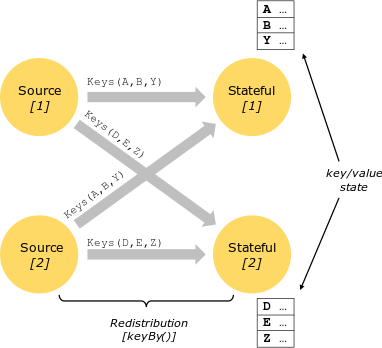
\includegraphics[width=0.5\columnwidth]{tecnologieUtilizzate/flink/state_partitioning.png} 
    \caption{Parallelizzazione del processamento del flusso per chiave in \textit{Apache Flink}}
\end{figure}

\myParagraph{Checkpoint}\label{sec:checkpoint}
Durante l'elaborazione dei dati possono avvenire degli errori che non permettono la continuità del processamento dei dati. \textit{Flink} permette di essere tollerante a questi errori tramite il meccanismo di \textbf{\textit{checkpoint}}. Un \textit{checkpoint} contrassegna un punto specifico in ciascuno dei flussi di \textit{input} insieme allo stato corrispondente per ciascuno degli operatori. Un flusso di dati in \textit{streaming} può essere ripreso da un \textit{checkpoint} mantenendo la coerenza (cioè elaborando il dato esattamente una volta) ripristinando lo stato degli operatori e riproducendo i \textit{record} dal punto prefissato dal \textit{checkpoint}.\\
Durante il processamento, in caso di errori (come errori di rete), \textit{Flink} interrompe il flusso di dati in \textit{streaming} ed esegue le seguenti operazioni:
\begin{itemize}
	\item{Il sistema riavvia gli operatori e li reimposta sull'ultimo \textit{checkpoint} riuscito;}
	\item{I flussi di \textit{input} vengono reimpostati al dato \gls{snapshot} dello stato.}
\end{itemize}
Inoltre viene garantito che tutti i \textit{record} elaborati come parte del flusso di dati parallelo riavviato non abbiano influito sullo stato del \textit{checkpoint} precedente.
Il meccanismo di \textit{checkpoint} (sia a livello di creazione che di ripristino da esso), se configurato durante l'elaborazione, è totalmente gestito da \textit{Flink}, rendendolo trasparente per l'utente.

\myParagraph{Savepoint}
Tutti i programmi che utilizzano il \textit{checkpoint} possono riprendere l'esecuzione da un \textbf{\textit{savepoint}}. I \textit{savepoint} consentono di aggiornare sia i programmi (quindi la logica al loro interno), che il \gls{cluster} di \textit{Flink}.\\
I \textit{savepoint} si possono considerare come dei veri e propri \textit{checkpoint}, che acquisiscono uno \gls{snapshot} del programma e lo scrivono in un \textit{back-end} di stato. I \textit{savepoint} si affidano al normale meccanismo di \textit{checkpoint}, descritto nella sezione \S\ref{sec:checkpoint}, per fare ciò. La differenza sostanziale con un \textit{checkpoint} è che il \textit{savepoint}:
\begin{itemize}
	\item{viene creato manualmente dall'utente;}
	\item{non viene eliminato quando viene eseguito un \textit{checkpoint} in un dato istante successivo al \textit{savepoint}.}
\end{itemize}


\subsection{Serializzazione}
Per salvare e ripristinare i dati durante la creazione di un \textit{checkpoint} o \textit{savepoint}, \textit{Flink} serializza e deserializza i dati in formato binario. Questo rende comprensibile il formato dei dati in qualunque sistema di gestione di essi.\\
\textit{Flink} pone alcune restrizioni sul tipo di elementi che possono trovarsi in un \textit{DataSet} o \textit{DataStream}. La ragione di ciò è che il sistema analizza i tipi per determinare strategie di esecuzione più efficienti.\\
La \gls{serializzazione} predefinita di \textit{Apache Flink} può essere suddivisa approssimativamente nei seguenti gruppi:

\begin{itemize}
	\item{
Serializzatori speciali forniti da \textit{Flink} per i tipi base (primitive \textit{Java} e loro forma \textit{boxed}), \textit{array}, tipi compositi (\textit{tuple}, \textit{case class} di \textit{Scala}, \textit{Rows}) e alcuni tipi ausiliari (\textit{Option}, \textit{Either}, \textit{Lists}, \textit{Maps}, …);}
	\item{\gls{pojo}, cioè un tipo di classe che soddisfa i seguenti requisiti:
\begin{itemize}
	\item{la classe deve essere pubblica;}
	\item{deve avere un costruttore pubblico senza argomenti (costruttore predefinito);}
	\item{tutti i campi sono pubblici o devono essere accessibili tramite le funzioni \textit{getter} e \textit{setter};}
	\item{il tipo di un campo deve essere supportato da un serializzatore registrato.}
\end{itemize}}
	\item{Tipi generici, cioè tipi di dati definiti dall'utente che non sono riconosciuti come \gls{pojo} e quindi serializzati tramite \textit{Kryo} (\S\ref{sec:kryo}).}
\end{itemize}
In alternativa alla \gls{serializzazione} offerta internamente da \textit{Flink}, si possono creare anche dei serializzatori personalizzati definiti dall'utente, i quali possono integrare altri sistemi di \gls{serializzazione} come per esempio \textbf{\textit{Avro}} (\S\ref{sec:avro}). I serializzatori personalizzati sono molto importanti per quanto riguarda lo \textbf{\textit{State Schema Evolution}}, infatti le applicazioni \textit{streaming} di \textit{Apache Flink} sono generalmente progettate per funzionare a tempo indeterminato o per lunghi periodi di tempo. Come per tutti i servizi di lunga durata, le applicazioni devono essere aggiornate per adattarsi alle mutevoli esigenze. Questo vale anche per gli schemi di dati su cui lavorano le applicazioni, i quali si evolvono insieme all'applicazione stessa.\\
Di seguito vengono analizzati i due \gls{framework} di \gls{serializzazione} citati precedentemente.

\myParagraph{Kryo}\label{sec:kryo}
\textit{Flink} utilizza il \gls{framework} \textit{Kryo} in modo totalmente trasparente per l'utente programmatore sui tipi di dati non riconosciuti come \gls{pojo} o che non sono corredati da serializzatori speciali. Se si utilizza \textit{Kryo}, è importante registrare il tipo di classe per permettere a \textit{Kryo} di memorizzare tale classe in modo che, durante la \gls{serializzazione}, \textit{Kryo} non debba aggiungere i nomi di classe completi come prefisso nel modulo serializzato. \textit{Kryo} usa questo meccanismo di \textit{tag} (interi) per identificare le classi sottostanti e ridurre il sovraccarico della \gls{serializzazione}.



\myParagraph{Avro}\label{sec:avro}
\textit{Flink} offre supporto per il \gls{framework} di \gls{serializzazione} \textit{Apache Avro} tramite la dipendenza \textit{org.apache.flink:flink-avro}. L'\textit{AvroSerializer} di \textit{Flink} può quindi sfruttare le prestazioni e la flessibilità di \textit{Avro}, soprattutto in termini di evoluzione dello schema quando le classi cambiano nel tempo.

\subsection{Testing}\label{sec:flink-testing}
\textit{Flink} espone delle funzionalità interne per permettere la stesura di \textbf{test di unità} relativi ad operatori \gls{stateful} o che utilizzano \textit{timer} e operatori \gls{stateless}. \textit{Apache Flink} offre, inoltre, la funzionalità di \textit{testing} relativa ad un intero \gls{cluster}. Per semplicità, all'interno di questa sezione viene esplicitata la procedura di creazione di un test di unità relativo ad un operatore \gls{stateful}, nonché l'unico tipo di test utilizzato durante il progetto.\\
Il \textit{testing} della funzionalità di un operatore che fa uso di uno stato o di un \textit{timer} implica testare l'interazione tra il codice prodotto dallo sviluppatore e il \textit{runtime} di \textit{Flink}. Per semplificare ciò \textit{Apache Flink} fornisce una raccolta di cosiddetti \textit{test harnesses}, i quali permettono di testare differenti operatori del tipo:
\begin{itemize}
	\item{\textbf{\textit{OneInputStreamOperatorTestHarness}:} per operatori di tipo \textit{DataStreams};}
	\item{\textbf{\textit{KeyedOneInputStreamOperatorTestHarness}:} per operatori di tipo \textit{KeyedStreams};}
	\item{\textbf{\textit{TwoInputStreamOperatorTestHarness}:} per operatori di tipo \textit{ConnectedStreams} di due \textit{DataStreams};}
	\item{\textbf{\textit{KeyedTwoInputStreamOperatorTestHarness}:} per operatori di tipo \textit{ConnectedStreams} di due \textit{KeyedStreams}.}
\end{itemize}

Il funzionamento dei \textit{test harnesses} prevede l'inserimento di \textit{record} nei differenti flussi trattati dall'operatore, il processamento di \textit{watermark} e il controllo riguardo al tempo di esecuzione (\textit{timer}) dell'operatore stesso. Inoltre è possibile fare asserzioni sugli stati interni e sull'\textit{output} dell'operatore, inclusi i \textit{side outputs}. 



%**************************************************************
\section{Scala}\label{sec:scala}
Il linguaggio di programmazione utilizzato all'interno del \gls{framework} \textit{Flink} è \textbf{Scala}. \textit{Scala} (da \textit{Scalable Language}) è un linguaggio di programmazione multi-paradigma studiato per integrare le caratteristiche e funzionalità dei \textbf{linguaggi orientati agli oggetti} e dei \textbf{linguaggi funzionali}. La compilazione di codice sorgente \textit{Scala} produce \textit{Java bytecode} per l'esecuzione su una \gls{jvm}. L'esecuzione di un programma prodotto in linguaggio \textit{Scala} avviene tramite \gls{jre}, il quale semplifica l'integrazione con le applicazioni e le componenti \textit{Java}.\\
Una delle peculiarità più importanti di \textit{Scala}, come accennato in precedenza, è l'integrazione di due paradigmi di programmazione molto noti:
\begin{itemize}
	\item{\textbf{Orientamento agli oggetti:} ogni elemento del linguaggio è un oggetto, inclusi numeri e funzioni che, così, possono essere memorizzate in variabili, essere passate come parametri, rappresentare il risultato di una chiamata di metodo, oppure essere estese tramite ereditarietà;}
	\item{\textbf{Funzionale:} ogni funzione è un valore. \textit{Scala} fornisce un linguaggio molto diretto per definire funzioni anonime (dichiarate e usate senza essere legate ad un nome), supporta funzioni di ordine superiore, permette alle funzioni di essere annidate e supporta funzioni parziali.}
\end{itemize}
Di seguito vengono elencate alcune strutture logiche specifiche di \textit{Scala} considerate importanti e differenti rispetto ai linguaggi di programmazione più conosciuti:
\begin{itemize}
	\item{\textbf{Case class:} le \textit{case class} vengono utilizzate principalmente per la modellazione di dati immutabili. A differenza delle \textit{class}, per istanziare una \textit{case class} non è necessaria la parola \textit{new} e le funzioni \textit{getter} sono automaticamente definite per i parametri del costruttore. Inoltre la comparazione fra \textit{case class} avviene per valori e non per riferimenti, cioè oggetti diversi ma con valori uguali sono considerati eguali;}
	\item{\textbf{Option:} come si evince dal nome, le \textit{Option} di \textit{Scala} sono utilizzate per rappresentare un tipo opzionale, cioè che contiene un valore del tipo specificato oppure no. Se un valore è presente, l'istanza dell'\textit{Option} sarà di tipo \textit{Some(x)}, dove \textit{x} rappresenta il valore del tipo specificato dall'\textit{Option} stessa. Se, invece, il valore non è presente, l'istanza rappresenterà un tipo \textit{None}.}
\end{itemize}
Un'altra caratteristica fondamentale di \textit{Scala} è quella di permettere l'utilizzo dell'astrazione dei tipi. Questo significa che l'utente non è tenuto a specificare nel codice il tipo dei parametri rappresentati, ma vengono dedotti dal contesto tramite il compilatore.


%**************************************************************

\section{ScalaTest}\label{sec:scala-test}
\textit{ScalaTest} è un \gls{framework} per la creazione di test basati sul linguaggio \textit{Scala} o \textit{Java}. \textit{ScalaTest} supporta diversi stili di test, ciascuno progettato per soddisfare un particolare insieme di esigenze. Di seguito viene rappresentato un esempio dello stile \textit{FlatSpec}, stile che è stato utilizzato per la redazione dei test di unità all'interno del progetto:

\begin{minted}{scala}
class SetSpec extends AnyFlatSpec {

  "An empty Set" should "have size 0" in {
    assert(Set.empty.size == 0)
  }

  it should "produce NoSuchElementException when head is invoked" in {
    assertThrows[NoSuchElementException] {
      Set.empty.head
    }
  }
}
\end{minted}

Nello stile \textit{FlatSpec} i nome dei test devono essere scritti secondo la convenzione: "\textit{X should Y}" e/o "\textit{A must B}".\\
Inoltre \textit{ScalaTest} offre i principali costrutti per la progettazione di test come per esempio \textit{Before} e \textit{After}, dove rispettivamente al loro interno viene  prodotto il codice che verrà eseguito prima e dopo di ogni test.

%**************************************************************
\section{Go}\label{sec:go}
Il linguaggio di programmazione utilizzato per la stesura delle \gls{api} è \textbf{\textit{Go}}.\\
\textit{Go}, conosciuto anche come \textit{Golang}, è un linguaggio di programmazione compilato e tipizzato staticamente, sintatticamente simile al linguaggio di programmazione \textit{C} eccetto per la dichiarazione dei tipi e per la mancanza di parentesi tonde nei costrutti \textit{for} e \textit{if}. Si differenzia dal linguaggio \textit{C}, inoltre, nel soddisfare esigenze di programmazione concorrente e nell'utilizzare un sistema di \textit{garbage collection} che si occupa autonomamente della gestione della memoria.\\
\textit{Go} è stato progettato per garantire una compilazione efficiente, un'esecuzione veloce e la facilità di programmazione.
\textit{Go} garantisce il supporto nativo nel linguaggio di numerose funzionalità dove altri linguaggi richiedono un \gls{framework} esterno, come per esempio la funzionalità di \textit{testing} del codice.

%**************************************************************
\section{IntelliJ IDEA}
\textit{IntelliJ IDEA} è un ambiente di sviluppo integrato (\gls{ide}) utilizzato prevalentemente per il linguaggio di programmazione \textit{Java}. Sviluppato da \textit{JetBrains} (prima conosciuto come \textit{IntelliJ}), è disponibile sia in licenza \textit{Apache} che in edizione proprietaria commerciale.\\
\textit{IntelliJ IDEA} offre numerose \textit{features} per facilitare lo sviluppo applicativo:
\begin{itemize}
	\item{\textbf{Codifica assistita:} l'\gls{ide} offre il completamento assistito del codice tramite l'analisi del contesto, la navigazione interna del codice che permette di passare da una classe o una parte di codice ad un'altra e il \textit{refactor} del codice stesso;}
	\item{\textbf{Integrazione di \textit{tools} esterni}: viene offerto l'integrazione con numerosi strumenti esterni come quelli relativi al \textit{build/packaging} e quelli relativi al versionamento del codice. In particolare durante la realizzazione del progetto è stato utilizzato il \textit{tool} \textbf{SBT} come strumento di \textit{build/packaging} e \textbf{GIT} come versionatore del codice;}
	\item{\textbf{Supporto a numerosi linguaggi di programmazione}: in particolare per la realizzazione del progetto è stato utilizzato un \textit{plugin} offerto da \textit{IntelliJ IDEA} per la codifica tramite il linguaggio \textbf{Scala} (\S\ref{sec:scala}).}
\end{itemize}

             % Strumenti utilizzati
% !TEX encoding = UTF-8
% !TEX TS-program = pdflatex
% !TEX root = ../tesi.tex

%**************************************************************
\chapter{Analisi dei requisiti}
\label{cap:analisi-requisiti}
%**************************************************************

\intro{Il capitolo contiene la rappresentazione dei casi d'uso per l'inserimento dei dati relativi alla configurazione del flusso di \textit{anomaly detection} e l'analisi dei requisiti effettuata per la realizzazione delle nuove funzionalità all'interno dell'applicativo \textit{SYN}. Il capitolo è strutturato suddividendo i requisiti in aree di sviluppo (operatori e API), questo per garantire un'analisi di essi più mirata.}\\


\section{Casi d'uso}

Per lo studio dei casi di utilizzo del prodotto sono stati creati dei diagrammi.
I diagrammi dei casi d'uso (in inglese \emph{Use Case Diagram}) sono diagrammi di tipo \gls{uml} dedicati alla descrizione delle funzioni o servizi offerti da un sistema, così come sono percepiti e utilizzati dagli attori che interagiscono col sistema stesso.
Essendo il progetto finalizzato alla creazione di un tool per l'automazione di un processo, le interazioni da parte dell'utilizzatore devono essere ovviamente ridotte allo stretto necessario. Per questo motivo i diagrammi d'uso risultano semplici e in numero ridotto.

\section{Classificazione dei requisiti}
I requisiti individuati sono identificati secondo la seguente codifica:
\begin{center}
\textbf{R[Importanza][Tipologia][CodicePadre].\{CodiceFiglio\}}\\
\end{center}
dove:


\begin{itemize}
\item {\textbf{Importanza}: rappresenta l'importanza del requisito e può essere:
	\begin{itemize}
	\item {\textbf{O (Obbligatorio)}: irrinunciabile per garantire il funzionamento richiesto;}
	\item {\textbf{D (Desiderabile)}: non strettamente necessario ma a valore aggiunto riconoscibile;}
	\item {\textbf{F (Facoltativo)}: relativamente utile oppure contrattabile a posteriori nel progetto.}
	\end{itemize}
}
\item{\textbf{Tipologia}: rappresenta il tipo di requisito e può essere:
\begin{itemize}
\item \textbf{F (Funzionale)}: descrive le funzionalità  offerte dall'applicativo;
\item \textbf{V (Vincolo)}: descrive i vincoli che l'applicativo è tenuto a rispettare.
\end{itemize}}
\item \textbf{CodicePadre}: rappresenta il codice di un requisito generico;
\item \textbf{CodiceFiglio} (opzionale): rappresenta il codice di un sotto caso di requisito;
\end{itemize}


\section{Requisiti operatore Bumblebee}
\subsection{Requisiti Funzionali}
{
\centering
\begin{longtable}{L{3cm} L{3cm} L{7.5cm}}
\caption{Requisiti Funzionali dell'operatore \textit{Bumblebee}}\\
\textbf{Identificativo} &
\textbf{Classificazione}&
\textbf{Descrizione}\\
\endhead
\hline

ROF1 & Obbligatorio & L'operatore deve garantire un'\textit{output} informativo che possa trattare un'\textit{asset} singolo\\
\hline
ROF2 & Obbligatorio & L'operatore deve garantire un'\textit{output} informativo che possa trattare un agglomerato di \textit{asset}\\
\hline
ROF2.1 & Obbligatorio & L'operatore deve garantire un'\textit{output} informativo che possa trattare un agglomerato di \textit{asset} suddivisi per categoria\\
\hline
ROF2.2 & Obbligatorio & L'operatore deve garantire un'\textit{output} informativo che possa trattare un agglomerato di \textit{asset} suddivisa per un gruppo definito dall'utente\\
\hline
\end{longtable}
}

\subsection{Requisiti di Vincolo}
{
\centering
\begin{longtable}{L{3cm} L{3cm} L{7.5cm}}
\caption{Requisiti di Vincolo dell'operatore \textit{Bumblebee}}\\
\textbf{Identificativo} &
\textbf{Classificazione}&
\textbf{Descrizione}\\
\endhead
\hline

ROV1 & Obbligatorio & L'operatore deve garantire un unico tipo di \textit{output} informativo che possa adattarsi alla rappresentazione di \textit{asset} singoli o \textit{asset} agglomerati\\
\hline
\end{longtable}
}





\section{Requisiti operatore Windowing}
\subsection{Requisiti Funzionali}
{
\centering
\begin{longtable}{L{3cm} L{3cm} L{7.5cm}}
\caption{Requisiti Funzionali dell'operatore \textit{Windowing}}\\
\textbf{Identificativo} &
\textbf{Classificazione}&
\textbf{Descrizione}\\
\endhead
\hline

ROF1 & Obbligatorio & L'operatore deve garantire il l'aggregazione di \textit{asset} su se stessi\\
\hline
ROF2 & Obbligatorio & L'operatore deve garantire il raggruppamento di \textit{asset} diversi fra di loro\\
\hline
ROF2.1 & Obbligatorio & L'operatore deve garantire l'aggregazione di \textit{asset} diversi fra di loro\\
\hline
ROF2.2 & Obbligatorio & L'operatore deve garantire l'allineamento di \textit{asset} diversi fra di loro\\
\hline
ROF3 & Obbligatorio & L'operatore deve garantire la creazione di un \textit{output} informativo che rappresenti un raggruppamento di \textit{asset}\\
\hline
ROF3.1 & Obbligatorio & L'operatore deve garantire la creazione di un \textit{output} informativo che rappresenti un'aggregazione di \textit{asset} differenti fra di loro\\
\hline
ROF3.2 & Obbligatorio & L'operatore deve garantire la creazione di un \textit{output} informativo che rappresenti un allineamento di \textit{asset} differenti fra di loro\\
\hline
ROF4 & Obbligatorio & L'operatore deve garantire la collezione di eventi senza raggruppamento nel caso in cui la finestra temporale sia nulla\\
\hline
ROF5 & Obbligatorio & L'operatore deve garantire la gestione di eventi in anticipo rispetto la finestra temporale attuale\\
\hline
ROF5.1 & Obbligatorio & L'operatore garantisce l'inserimento di eventi in anticipo nella futura finestra temporale se esso è contenuto nei suoi limiti (inizio e fine)\\
\hline
ROF5.2 & Obbligatorio & L'operatore deve scartare eventi in anticipo se essi non sono contenuti nei limiti (inizio e fine) della futura finestra temporale\\
\hline
ROF5.2 & Obbligatorio & L'operatore deve porte scartare eventi in anticipo se essi non sono contenuti nei limiti (inizio e fine) della futura finestra temporale\\
\hline
ROF6 & Obbligatorio & L'operatore deve scartare eventi se non è presente nessuna configurazione per la finestra temporale attuale\\
\hline
ROF7 & Obbligatorio & L'operatore deve gestire l'inizio e la fine della prima finestra temporale in base al primo evento ricevuto\\
\hline
\end{longtable}
}

\subsection{Requisiti di Vincolo}




\section{Requisiti operatore AlertCoProcess}
\subsection{Requisiti Funzionali}
{
\centering
\begin{longtable}{L{3cm} L{3cm} L{7.5cm}}
\caption{Requisiti Funzionali dell'operatore \textit{AlertCoProcess}}\\
\textbf{Identificativo} &
\textbf{Classificazione}&
\textbf{Descrizione}\\
\endhead
\hline

ROF1 & Obbligatorio & L'operatore deve garantire un'\textit{output} informativo che possa trattare un'\textit{asset} singolo\\
ROF2 & Obbligatorio & L'operatore deve garantire un'\textit{output} informativo che possa trattare un agglomerato di \textit{asset}\\
ROF2.1 & Obbligatorio & L'operatore deve garantire un'\textit{output} informativo che possa trattare un agglomerato di \textit{asset} suddivisi per categoria\\
ROF2.2 & Obbligatorio & L'operatore deve garantire un'\textit{output} informativo che possa trattare un agglomerato di \textit{asset} suddivisa per un gruppo definito dall'utente\\
\hline
\end{longtable}
}

\subsection{Requisiti di Vincolo}

\section{Requisiti API di configurazione}
\subsection{Requisiti Funzionali}

\subsection{Requisiti di Vincolo}





\begin{figure}[!h] 
    \centering 
    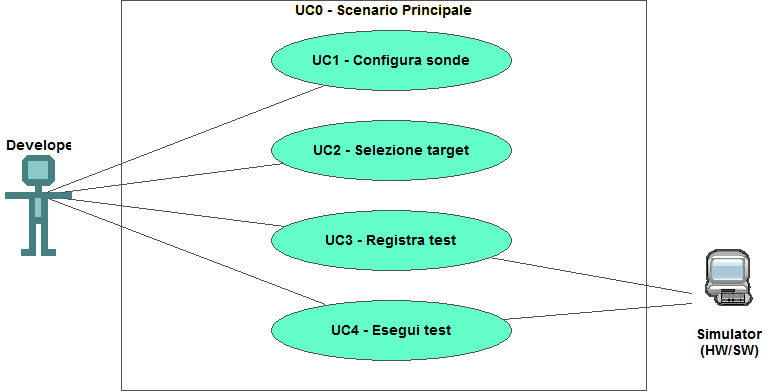
\includegraphics[width=0.9\columnwidth]{usecase/scenario-principale} 
    \caption{Use Case - UC0: Scenario principale}
\end{figure}

\begin{usecase}{0}{Scenario principale}
\usecaseactors{Sviluppatore applicativi}
\usecasepre{Lo sviluppatore è entrato nel plug-in di simulazione all'interno dell'IDE}
\usecasedesc{La finestra di simulazione mette a disposizione i comandi per configurare, registrare o eseguire un test}
\usecasepost{Il sistema è pronto per permettere una nuova interazione}
\label{uc:scenario-principale}
\end{usecase}

\section{Tracciamento dei requisiti}

Da un'attenta analisi dei requisiti e degli use case effettuata sul progetto è stata stilata la tabella che traccia i requisiti in rapporto agli use case.\\
Sono stati individuati diversi tipi di requisiti e si è quindi fatto utilizzo di un codice identificativo per distinguerli.\\
Il codice dei requisiti è così strutturato R(F/Q/V)(N/D/O) dove:
\begin{enumerate}
	\item[R =] requisito
    \item[F =] funzionale
    \item[Q =] qualitativo
    \item[V =] di vincolo
    \item[N =] obbligatorio (necessario)
    \item[D =] desiderabile
    \item[Z =] opzionale
\end{enumerate}
Nelle tabelle \ref{tab:requisiti-funzionali}, \ref{tab:requisiti-qualitativi} e \ref{tab:requisiti-vincolo} sono riassunti i requisiti e il loro tracciamento con gli use case delineati in fase di analisi.

\newpage

\begin{table}[hbt!]
\caption{Tabella del tracciamento dei requisti funzionali}
\label{tab:requisiti-funzionali}
\begin{tabularx}{\textwidth}{lXl}
\hline\hline
\textbf{Requisito} & \textbf{Descrizione} & \textbf{Use Case}\\
\hline
RFN-1     & L'interfaccia permette di configurare il tipo di sonde del test & UC1 \\
\hline
\end{tabularx}
\end{table}%

\begin{table}[hbt!]
\caption{Tabella del tracciamento dei requisiti qualitativi}
\label{tab:requisiti-qualitativi}
\begin{tabularx}{\textwidth}{lXl}
\hline\hline
\textbf{Requisito} & \textbf{Descrizione} & \textbf{Use Case}\\
\hline
RQD-1    & Le prestazioni del simulatore hardware deve garantire la giusta esecuzione dei test e non la generazione di falsi negativi & - \\
\hline
\end{tabularx}
\end{table}%

\begin{table}[hbt!]
\caption{Tabella del tracciamento dei requisiti di vincolo}
\label{tab:requisiti-vincolo}
\begin{tabularx}{\textwidth}{lXl}
\hline\hline
\textbf{Requisito} & \textbf{Descrizione} & \textbf{Use Case}\\
\hline
RVO-1    & La libreria per l'esecuzione dei test automatici deve essere riutilizzabile & - \\
\hline
\end{tabularx}
\end{table}%             % Analisi dei requisiti
% !TEX encoding = UTF-8
% !TEX TS-program = pdflatex
% !TEX root = ../tesi.tex

%**************************************************************
\chapter{Progettazione e codifica}
\label{cap:progettazione-codifica}
%**************************************************************

\intro{Tale capitolo descrive in dettaglio la struttura del progetto, la progettazione e codifica delle nuove funzionalità, nonchè l'integrazione di esse con la struttura preesistente. La fase di progettazione e codifica non sono intese come attività prettamente distinte, infatti alcune analisi effettuate durante la progettazione iniziale antecedente alla codifica sono risultate non sufficienti a coprire numerose casistiche sorte durante lo sviluppo effettivo, per cui è stato necessario una riprogettazione mirata a risolvere le problematiche sorte.}

\section{Adattamento degli operatori preesistenti}
Durante l'analisi preventiva dei rischi relativa alle nuove funzionalità, sono sorti subito dei problemi relativi all'adattabilità degli operatori preesistenti con la nuove funzionalità create. Tali problematiche di adattabilità si possono riassumere in micro-aree:

\begin{itemize}
	\item{adattabilità della rappresentazione degli eventi tramite l'\textit{output} dell'\textbf{operatore \textit{Bumblebee}} definito come \textbf{\textit{BumblebeeOutput}}, che va a definire la trasformazione degli eventi "grezzi" in eventi arricchiti da informazioni necessarie per il loro processamento;}
	\item{adattabilità dell'\textbf{operatore \textit{Windowing}} che ora non deve solo trattare aggregazione di eventi ricevuti dallo stesso tipo di risorsa, ma deve gestire l'aggregazione e/o l'allineamento anche di risorse di tipo differente per permettere all'operatore \textit{AlertCoProcess} di eseguire un controllo a livello di insieme relativo a risorse differenti;}
	\item{adattabilità dell'\textbf{operatore \textit{AlertCoProcess}} per permettere ad esso di gestire e di controllare gruppi di eventi derivanti da risorse non più eguali fra di loro. Quindi di gestire il controllo relativo alla presenza di una anomalia relativa ad un gruppo di risorse. Inoltre, tale operatore, deve adattarsi anche alla presenze di due nuovi \textit{detector} di anomalie, quali \textbf{\textit{Unsupervised}} e \textbf{\textit{Rule based}}.}
\end{itemize}
	
Nello specifico si va ad analizzare le modifiche adottate riguardo le tre micro-aree descritte precedentemente.

%**************************************************************

\section{Operatore Bumblebee}\label{sec:bbout}
Per permettere la rappresentazione di gruppi di risorse differenti, viene cambiata la struttura dell'\textit{output} dell'operatore \textbf{\textit{Bumblebee}}, rappresentato inizialmente in un formato \gls{json} così formato:

\begin{minted}{js}
{
  "id": // id dell'evento, generato o trasformato dall'evento originale, in formato String,
  "pipeID": // id della pipeline, in formato String,
  "pipeVersion": //versione della pipeline, in formato String,
  "adapterID": //id dell'adattatore, in formato String,
  "tid": //id del cliente, in formato String,
  "assetID": //id della risorsa, in formato String,
  "ts": //timestamp dell'evento, in formato String,
  "asset": //informazioni relative alla risorsa dopo che è stata arricchita, in formato AssetInfo
  "data": //payload dei dati dell'evento trasformati in formato JSON,
  "ctxData": //dati relativi al contesto, come per esempio il tempo metereologico, in formato JSON,
  "meta": //metadati arricchiti dall'operatore di anomaly detection, in formato Option[EventMeta],
  "type": //tipo di BumblebeeOutput", in formato Option[String],
  "srcID": //id della fonte dell'evento in formato String
}
\end{minted}

Dopo l'opportuna modifica, la struttura rappresentate il \textbf{\textit{BumblebeeOutput}} risulta la seguente:

\begin{minted}{js}
{
  "id": // id dell'evento, generato o trasformato dall'evento originale, in formato String,
  "pipeID": // id della pipeline, in formato String,
  "pipeVersion": //versione della pipeline, in formato String,
  "adapterID": //id dell'adattatore, in formato String,
  "tid": //id del cliente, in formato String,
  "subject": {
	  "id": //id dell'oggetto, in formato String,
	  "type": //tipo dell'oggetto rapresentanto (asset,category,group), in formato String
  }
  "ts": //timestamp dell'evento, in formato String,
  "asset": //informazioni relative alla risorsa dopo che è stata arricchita, in formato AssetInfo
  "data": //payload dei dati dell'evento trasformati in formato JSON,
  "ctxData": //dati relativi al contesto, come per esempio il tempo metereologico, in formato JSON,
  "meta": //metadati arricchiti dall'operatore di anomaly detection, in formato Option[EventMeta],
  "type": //tipo di BumblebeeOutput", in formato Option[String],
  "srcID": //id della fonte dell'evento in formato String
}
\end{minted}
dove la rappresentazione è slegata da un \textit{asset} (risorsa) specifico. Per cui l'\textit{output} sarà adattato ad un \textbf{soggetto} generale, rappresentato da un proprio \textbf{\textit{id}} e da un suo \textbf{tipo}.
Tale struttura finale garantisce un corretto processamento del dato nel caso in cui si tratti di una risorsa singola oppure di un raggruppamento di quest'ultime.

%**************************************************************

\section{Operatore Windowing}
L'\textbf{operatore \textit{Windowing}} serve per rappresentare un determinato evento in una data finestra temporale. Inizialmente, tale operatore, trattava l'aggregazione solo di una determinata \textbf{risorsa} su se stessa, cioè \textbf{sommando} o \textbf{mediando} un determinato valore. Ora in tale operatore non solo permane il comportamento appena descritto, ma è presente anche la funzionalità che si occupa di allineare e/o aggregare fra di loro risorse di tipo differente, per permettere un processamento dei dati a livello collettivo. Per definire il comportamento della finestra temporale, è necessaria un'apposita \textbf{configurazione} che sarà iniettata durante l'elaborazione attiva dei dati, per permetterne la modifica del comportamento senza dover riavviare l'intero applicativo e creare uno stallo in esso.\\
L'operatore \textit{Windowing} è una \textbf{\textit{KeyedCoProcessFunction}}, così definita:
\begin{minted}{scala}
class Windowing(outputTagValues: OutputTag[AnomalyStepConfigurationCommand]) extends KeyedCoProcessFunction[String, BumblebeeOutput, AnomalyStepConfigurationCommand, GroupedEvents] {
	// ...
  }
\end{minted}
Dove in entrata avrà due tipi di flussi, uno relativo agli eventi da raggruppare di tipo \textit{BumblebeeOutput} (\S\ref{sec:pr1-windowing}) e uno relativo alla configurazione dell'operatore di tipo \textit{AnomalyStepConfiguration} (\S\ref{sec:pr2-windowing}). Tale operatore opera su flussi suddivisi per chiave definita come \textit{pipeID}.\\
Il metodo che verrà richiamato alla fine di una specifica finestra temporale è il metodo \textit{onTimer} (\S\ref{sec:on-timer-windowing}), il quale collezionerà gli eventi all'interno della \textit{window} appena conclusa e programmerà l'inizio della successiva finestra temporale.

\subsection{Stati dell'operatore}\label{sec:stati-windowing}
Per permettere una corretta gestione di entrambi i flussi, l'operatore \textit{Windowing} sfrutta i seguenti \textbf{stati} interni:
\begin{itemize}
		\item{\textbf{\textit{cfg}:} l'attuale configurazione della finestra temporale;}
		\item{\textbf{\textit{mapToAggregator}:} mappa che gestisce gli aggregatori (\S\ref{sec:aggregator}), i quali sono mappati per l'\textit{id} del gruppo;}
		\item{\textbf{\textit{mapToListFutureEvents}:} mappa che gestisce la lista degli eventi arrivati in anticipo, i quali sono mappati per l'\textit{id} del gruppo;}
		\item{\textbf{\textit{windowBeginTs}:} l'inizio dell'attuale finestra temporale;}
		\item{\textbf{\textit{scheduledTimer}:} \textit{timer} schedulato per collezionare gli eventi visti dalla \textit{window}, il quale coincide con la fine dell'attuale finestra temporale;}
		\item{\textbf{\textit{pipeStatus}:} mappa che gestisce la versione delle varie \gls{pipeline}, le quali sono mappate per l'\textit{id} della \gls{pipeline}.}
\end{itemize}


\subsection{Flusso degli eventi da raggruppare}\label{sec:pr1-windowing}
Tale flusso è gestito dal metodo \textit{processElement1}, il quale è un metodo ereditato dalla classe \textbf{KeyedCoProcessFunction} e sovrascritto dalla classe rappresentate l'operatore (\textit{Windowing}). Il flusso attuale dell'operatore prevede questi \textit{step}:

\begin{enumerate}
	\item{arrivo dell'evento di tipo \textit{BumblebeeOutput};}
	\item{controllo relativo a se la configurazione è presente, nel caso in cui non sia presente si saltano tutti i passaggi successivi e l'evento viene ignorato;}
	\item{per ogni gruppo contenuto all'interno del filtro di aggregazione della \textit{window} verrà fatto il controllo per verificare che quel determinato gruppo è filtrato per accettare quel determinato evento in entrata;}
\item{se l'evento è contenuto all'interno del filtro di un gruppo, viene controllata se la durata della \textit{window} è nulla (minore o uguale a zero), in questa casistica l'evento viene collezionato all'interno della struttura dati rappresentata dal \textit{GroupedEvents} (\S\ref{sec:ge}) senza essere aggregato o allineato con altri eventi. Il flusso relativo all'evento entrante termina;}
\item{se la durata della \textit{window} ha una durata non nulla (maggiore di zero), l'evento verrà inserito nell'attuale \textit{window} se il suo \gls{timestamp} è contenuto nei limiti di essa (inizio e fine). Se, invece, l'evento è antecedente all'inizio della \textit{window}, viene scartato. Infine, se l'evento è successivo alla fine della finestra temporale, verrà inserito all'interno dello stato \textbf{\textit{mapToListFutureEvents}} (\S\ref{sec:stati-windowing}). Tale evento verrà trattato nella successiva \textit{window}.}
\end{enumerate}

Per gestire l'inizio di una determinata nuova finestra temporale (quindi basata su una nuova \textbf{configurazione} per essa) verrà fatto un controllo per definire se l'evento entrante è il primo a partire da una nuova configurazione. In questo caso l'inizio della \textit{window} è eguale al \gls{timestamp} dell'evento entrante e la fine della \textit{window} è equivalente alla somma dell'inizio della finestra temporale con la sua durata (definita nella configurazione).
\subsection{Flusso di configurazione della window}\label{sec:pr2-windowing}
Tale flusso è gestito dal metodo \textit{processElement2}, il quale è un metodo ereditato dalla classe \textbf{KeyedCoProcessFunction} e sovrascritto dalla classe rappresentate l'operatore (\textit{Windowing}). Il flusso attuale dell'operatore prevede questi \textit{step}:

\begin{enumerate}
	\item{arrivo dell'evento riguardate la configurazione di tipo \textit{AnomalyStepConfiguration};}
	\item{controllo relativo a se la configurazione è di tipo "\textit{update}" o "\textit{delete}". In caso la configurazione non rappresenti nessuno dei due casi appena citati il flusso termina collezionando l'evento in un \textit{SideOutput}, cioè un coda differente rispetto a quella principale relativa ai \textit{GroupedEvents} (\S\ref{sec:ge}). Tale coda tratta gli eventi di tipo \textit{AnomalyStepConfiguration};}
	\item{Nel caso in cui la configurazione comprenda uno dei due tipi citati nel punto precedente, verrà fatto un controllo per verificare che la configurazione \textbf{relativa alla \textit{window}} (che è contenuta all'interno della configurazione di tipo \textit{AnomalyStepConfiguration}) sia presente e sia diversa da quella precedente, il che significa che la configurazione precedente è inesistente o che quella precedente si differenzia da quella attuale per almeno una di queste condizioni:
	\begin{itemize}
		\item{differente durata della finestra temporale;}
		\item{differente metodo di aggregazione;}
		\item{differente lista di gruppi su cui lavorerà la \textit{window};}
		\item{differenti parametri \textbf{relativi ai dati degli eventi} su cui si andrà a fare l'aggregazione;}
		\item{differenti \textbf{parametri del contesto} relativi agli eventi su cui si andrà a fare l'aggregazione.}
	\end{itemize}
	
Se la configurazione della \textit{window} è differente da quella precedente, vengono svuotati i relativi stati dell'operatore su cui opera la finestra temporale, quali \textbf{\textit{mapToAggregator}}, \textbf{\textit{mapToListFutureEvents}}, \textbf{\textit{windowBeginTs}} e \textbf{\textit{scheduledTimer}}. Di seguito viene aggiornato lo stato \textbf{\textit{cfg}} con i dati della finestra temporale nuova.\\
Se, invece, la nuova configurazione della finestra temporale è equivalente a quella precedente, non viene fatto nulla.\\
Infine viene aggiornato lo \textbf{\textit{pipeStatus}}.\\
Per una descrizione approfondita degli stati dell'operatore \textit{Windowing} fare riferimento alla sezione \S\ref{sec:stati-windowing}.
}
\item{Se invece la \textbf{configurazione della \textit{window}} non esiste, verrano svuotati tutti gli stati presenti nella sezione \S\ref{sec:stati-windowing}.}
\end{enumerate}

\subsection{OnTimer}\label{sec:on-timer-windowing}
Il metodo \textbf{\textit{onTimer}} è colui che gestisce la logica al termine di ogni finestra temporale. Tale funzione si occupa di creare un \textit{GroupedEvents} (\S\ref{sec:ge}) collezionando gli eventi visti secondo le regole definite dalla configurazione e ha il compito di configurare la prossima \textit{window}. Il metodo segue questi \textit{step}:
\begin{enumerate}
	\item{controllo relativo a se la configurazione della finestra temporale è settata, in caso negativo vengono saltati tutti gli \textit{step} successivi;}
	\item{in base alla modalità di aggregazione definita nella configurazione della finestra temporale, per ogni \textbf{\textit{id} del gruppo} contenuto all'interno dello stato \textbf{\textit{mapToAggregator}} verrà creato e collezionato un \textit{GroupedEvents} (\S\ref{sec:ge}) contenente gli eventi aggregati o allineati secondo la modalità definita, la quale può essere:
	\begin{itemize}
		\item{\textbf{\textit{barrier}:} in questa modalità gli eventi vengono \textbf{allineati} e il metodo che si occupa di questa funzionalità è il metodo \textit{selfAggregate} dell'aggregatore;}
		\item{\textbf{\textit{aggregation\textunderscore sum}:} in questa modalità gli eventi vengono raggruppati in uno unico, per cui verrà creato un nuovo \textit{BumblebeeOutput} che come parametri avrà il \gls{json} ritornato dal metodo \textit{groupAggregateDataFields} dell'aggregatore;}
		\item{\textbf{\textit{aggregation\textunderscore mean}:} in questa modalità gli eventi vengono raggruppati in uno unico, per cui verrà creato un nuovo \textit{BumblebeeOutput} che come parametri avrà il \gls{json} ritornato dal metodo \textit{groupAggregateDataFields} dell'aggregatore.}
	\end{itemize}
	Per la logica specifica di aggregazione vedere la sezione \S\ref{sec:aggregator};}
	\item{Creazione della nuova finestra temporale, cui l'inizio e la fine sono impostati rispettivamente con il \gls{timestamp} che ha attivato il metodo \textit{onTimer} e tale \gls{timestamp} sommato alla durata della \textit{window}. Di seguito vengono rimossi gli aggregatori all'interno dello stato \textbf{\textit{mapToAggregator}} che non contengono eventi inseriti nello stato \textbf{\textit{mapToListFutureEvents}} (nel caso in cui siano presenti degli eventi futuri, verrà istanziato un nuovo aggregatore contente già questi eventi). Infine viene svuotato lo stato \textbf{\textit{mapToListFutureEvents}}.
	}
\end{enumerate}

\subsection{GroupedEvents}\label{sec:ge}
L'\textit{output} dell'operatore, dapprima rappresentava solo una \textbf{risorsa singola}, ora invece tratterà un \textbf{gruppo}, il quale è identificato da un \textbf{\textit{id}}, da un \textbf{\gls{timestamp}} e da un \textbf{\textit{array}} di risorse di tipo \textit{BumblebeeOutput}.\\
Il \textit{GroupedEvents} può rappresentare logicamente due tipi logici di dato:
\begin{itemize}
	\item{\textbf{singolo elemento aggregato:} dove l'\textit{array} degli eventi è formato da un singolo elemento, l'\textit{id} del gruppo equivale all'\textit{id} definito dalla configurazione e il \textit{\gls{timestamp}} equivale a quello definito durante l'aggregazione effettiva;}
	\item{\textbf{allineamento:} dove l'\textit{array} degli eventi è formato da \textit{N} elementi, l'\textit{id} del gruppo equivale all'\textit{id} definito dalla configurazione e il \textit{\gls{timestamp}} equivale a quello definito durante l'aggregazione effettiva.}
\end{itemize}

\subsection{Aggregatore}\label{sec:aggregator}
L'aggregatore è la componente che si occupa di aggregare o allineare gli eventi all'interno della finestra temporale. L'operatore \textit{Windowing}, come spiegato nella sezione \S\ref{sec:stati-windowing} avrà uno stato che mapperà ogni \textit{id} del gruppo al suo specifico aggregatore. L'aggregatore in questione è di tipo \textit{BboutAggregator}, che è una classe contenente i seguenti parametri:

\begin{itemize}
	\item{\textbf{\textit{selfAggregatorMode}:} definisce il tipo di aggregazione che verrà fatto sugli \textit{asset} equivalenti fra di loro;}
	\item{\textbf{\textit{groupAccumulatorMode}:} definisce il tipo di aggregazione che verrà eseguito su \textit{asset} all'interno dello stesso gruppo;}
	\item{\textbf{\textit{acc}:} struttura che gestisce la mappatura fra un particolare \textit{asset} con una mappa che per chiave ha il nome di uno specifico parametro su cui si vuole andare a fare l'aggregazione e per valore ha la lista dei valori di quel parametro visti fino a quel determinato momento;}
	\item{\textbf{\textit{dataFields}:} \textit{array} contente i parametri degli eventi su cui si vuole fare l'aggregazione, decisi all'interno della \textbf{configurazione della \textit{window}};}
	\item{\textbf{\textit{ctxDataFields}:} \textit{array} contente i parametri del contesto degli eventi su cui si vuole fare l'aggregazione, decisi all'interno della \textbf{configurazione della \textit{window}}}
\end{itemize}

I metodi principali che gestiscono l'aggregazione a livello di \textbf{\textit{asset}} e a livello di \textbf{gruppo} sono:

\begin{itemize}
	\item{\textbf{\textit{add}:} tale metodo si occupa di salvare i valori dei parametri relativi agli \textit{asset} entranti nell'operatore \textit{Windowing}, dove tali parametri sono la concatenazione di \textit{dataFields} e \textit{ctxDataFields}. Per cui ad ogni chiamata di tale metodo verrà passato un particolare evento di tipo \textit{BumblebeeOutput}, tramite l'\textit{id} dell'evento viene estratta la mappa corrispondente ai parametri di \textit{dataFields} e \textit{ctxDataFields} e verrà aggiunto il valore del determinato parametro alla \textbf{lista dei valori} se esso è contenuto all'interno dell'evento.\\
Alla fine viene aggiornato il parametro \textit{acc} con la mappa aggiornata contenente la lista dei valori arricchita del nuovo valore, se trovato;}
	\item{\textbf{\textit{selfAggregate}:} tale metodo si occupa della vera e propria aggregazione degli \textit{asset} \textbf{su se stessi}, cioè per ogni \textit{asset} all'interno della mappa \textit{acc} (dove l'\textit{asset} è la chiave stessa) verranno aggregati i valori contenuti nel parametro \textit{dataFields} e \textit{ctxDataFields} secondo il metodo di aggregazione definito da \textit{selfAggregatorMode}.\\
	Se un determinato parametro ha la lista dei rispettivi valori minore o uguale a zero, vuol dire che esso non è appartenuto allo specifico \textit{BumblebeeOutput} che si sta aggregando, perciò tale parametro \textbf{non} verrà aggiunto con un valore di default durante l'aggregazione.\\
	Come tipo di ritorno tale metodo ritornerà un \textit{array} di \textit{BumbleebeeOutput} dove ogni \textit{asset} avrà i parametri interni a \textit{dataFields} e \textit{ctxDataFields} aggregati secondo il metodo definito e i parametri non interni ai due \textit{array} appena citati valorizzati con l'ultimo elemento visto di quel parametro. Se un determinato \textbf{asset} non contiene nessuno \textit{dataField}, non viene aggiunto all'\textit{array} ritornato;}
	\item{\textbf{\textit{groupAggregateDataFields}:} tale metodo si occupa di aggregare i parametri all'interno di \textit{asset} diversi fra di loro aggregati precedentemente su se stessi tramite il metodo \textit{selfAggregate}. Per ogni parametro contenuto nell'\textit{array} all'interno di \textit{dataFields} viene fatta l'aggregazione dei valori di quel determinato parametro all'interno dei \textit{BumblebeeOutput} ritornati dal metodo \textit{selfAggregate}. Il metodo ritorna un \gls{json} contenente l'aggregazione dei parametri contenuti in \textit{dataFields} secondo il metodo definito in \textit{groupAccumulatorMode}. Se un determinato parametro non è contenuto in almeno un \textit{BumblebeeOutput}, viene ritornato un \gls{json} vuoto, per permettere all'operatore di \textit{Windowing} di poter saltare la collezione del \textit{groupedEvents} che verrebbe creato.}
\end{itemize}



%**************************************************************
\section{Operatore AlertCoProcess}
L'operatore \textbf{\textit{AlertCoProcess}} è colui che si occupa di sollevare segnalazioni nel caso sia presente un'anomalia riguardo l'evento entrante di tipo \textit{GroupedEvents} (\S\ref{sec:ge}). Dapprima l'\textit{AlertCoProcess} lavorava solo su un tipo di evento legato ad una risorsa singola, mappando l'\textit{id} del \textit{detector} ad un'altra mappa dove la chiave è rappresentata dall'\textit{id} della risorsa e il valore è rappresentato dal vero e proprio \textit{detector}.\\
Ora, invece, la struttura è basata sull'\textit{id} del gruppo, per cui è stata creata un'ulteriore mappa fra \textit{id} del gruppo e \textit{id} del \textit{detector}, inoltre la chiave della mappa interna non è più rappresentata da un'\textit{id} della risorsa, ma da un \textit{id} del soggetto dopo la modifica di \textit{Bumblebee} (\S\ref{sec:bbout}).\\
L'operatore \textit{AlertCoProcess} è una \textbf{\textit{KeyedCoProcessFunction}}, così definita:
\begin{minted}{scala}
class AlertCoProcess (inspectionTag: OutputTag[MongoInsertDocument]) extends KeyedCoProcessFunction[String, GroupedEvents, AnomalyStepConfigurationCommand, (String, BumblebeeOutput)] {
	// ...
  }
\end{minted}
Dove in entrata avrà due tipi di flussi, uno relativo agli eventi su cui controllare se viene rilevata un'anomalia di tipo \textit{GroupedEvents} (\S\ref{sec:pr1-alertcoprocess}) e uno relativo alla configurazione dell'operatore di tipo \textit{AnomalyStepConfiguration} (\S\ref{sec:pr2-alertcoprocess}). Tale operatore opera su flussi suddivisi per chiave definita come \textit{pipeID}.\\
L'operatore lavora su un singolo tipo di \textit{detector}, il quale è legato indirettamente al \textit{pipeID}. Anche se il tipo di \textit{detector} è lo stesso, la configurazione dei parametri utilizzati da esso può cambiare a seconda del tipo gruppo che viene definito all'interno del \textit{GroupedEvents} entrante.


\subsection{Stati dell'operatore}\label{sec:stati-alertcoprocess}
Per permettere una corretta gestione di entrambi i flussi, l'operatore \textit{AlertCoProcess} sfrutta i seguenti \textbf{stati} interni:
\begin{itemize}
		\item{\textbf{\textit{isGroupingDetector}:} valore \textit{booleano} che identifica se il \textit{detector} dell'operatore tratta gli eventi come gruppo o no;}
		\item{\textbf{\textit{tid}:} identifica il cliente all'interno dell'\textit{AlertCoProcess};}
		\item{\textbf{\textit{mapToDetectorID}:} mappa che gestisce la correlazione fra l'\textit{id} del gruppo (chiave) e l'\textit{id} del \textit{detector} (valore);}
		\item{\textbf{\textit{mapToDetector}:} mappa che gestisce la correlazione fra il l'\textit{id} del \textit{detector} (chiave) e un ulteriore mappa (valore) che lega l'\textit{id} di un \textbf{soggetto}/\textbf{gruppo} con il suo vero e proprio \textit{detector};}
		\item{\textbf{\textit{detectorsConfigs}:} l'attuale configurazione del tipo di \textit{detector};}
		\item{\textbf{\textit{pipeStatus}:} mappa che gestisce la versione delle varie \gls{pipeline}, le quali sono mappate per l'\textit{id} della \gls{pipeline}.}
\end{itemize}

\subsection{Flusso degli eventi da controllare}\label{sec:pr1-alertcoprocess}
Tale flusso è gestito dal metodo \textit{processElement1}, il quale è un metodo ereditato dalla classe \textbf{KeyedCoProcessFunction} e sovrascritto dalla classe rappresentate l'operatore (\textit{AlertCoProcess}). Il flusso attuale dell'operatore prevede questi \textit{step}:
\begin{enumerate}
	\item{arrivo dell'evento di tipo \textit{GroupedEvents};}
	\item{viene estratta la mappa dei \textit{detector} tramite l'\textit{id} del \textit{detector}, estratto rispettivamente tramite l'\textit{id} del \textit{gruppo}. Ovviamente vengono effettuati dei controlli per verificare l'esistenza delle chiavi all'interno delle due mappe;}
	\item{se lo stato \textbf{\textit{isGroupingDetector}} ha come valore \textit{true}, vuol dire che l'anomalia, se presente, deve essere sollevata sul gruppo. Per cui viene estratto l'unico \textit{detector} (tramite l'\textit{id} del gruppo) dalla mappa estratta dallo \textit{step} precedente. Se il \textit{detector} è presente si utilizza quello preesistente, altrimenti ne viene creato uno nuovo. Infine viene creato un \textit{BumblebeeOutput} rappresentativo del gruppo su cui si sollevare la possibile anomalia rilevata dal \textit{detector};}
	\item{se lo stato \textbf{\textit{isGroupingDetector}}, invece, ha come valore \textit{false}, vuol dire che l'anomalia deve essere alzata su un singolo evento. Per cui per ogni evento interno all'\textit{array} degli eventi contenuto nell'oggetto \textit{GroupedEvents}, verrà estratto il \textit{detector} contenuto all'interno della mappa estratta nel punto 2. Su questo \textit{detector} viene controllato se è di tipo \textit{single input} (accetta un solo evento in entrata) oppure \textit{multiple input} (accetta un \textit{array} di eventi in entrata). A seconda dei due casi appena citati verrà passato o il singolo evento da cui si è estratto lo specifico \textit{detector} oppure tutto l'\textit{array} degli eventi. Nonostante ciò la possibile anomalia verrà rilevata sull'evento a cui è mappato il \textit{detector}.}
\end{enumerate}

\subsection{Flusso di configurazione dell'AlertCoProcess}\label{sec:pr2-alertcoprocess}
Tale flusso è gestito dal metodo \textit{processElement2}, il quale è un metodo ereditato dalla classe \textbf{KeyedCoProcessFunction} e sovrascritto dalla classe rappresentate l'operatore (\textit{AlertCoProcess}). Il flusso attuale dell'operatore prevede questi \textit{step}:

\begin{enumerate}
	\item{arrivo dell'evento di tipo \textit{AnomalyStepConfigurationCommand};}
	\item{la configurazione può essere di tre tipi differenti:
	\begin{itemize}
		\item{\textbf{\textit{update}:} in questo caso è richiesto l'aggiornamento dei \textit{detector}. Per ogni \textit{detector configuration} contenuto all'interno della nuova configurazione viene estratto l'\textit{id} del \textit{detector}, con il quale viene verificato se esso è presente all'interno dello stato \textbf{\textit{mapToDetectorID}}. Nel caso in cui l'\textit{id} del \textit{detector} sia contenuto all'interno della mappa verrà fatto l'accesso alla lista relativa di tutti i veri e propri \textit{detector} collegati a quel determinato \textit{id}. Per cui ogni \textit{detector} verrà aggiornato secondo la nuova configurazione fornita. La modalità di aggiornamento del \textit{detector} è specificata nella sezione \S\ref{sec:detector-alertcoprocess}. Nel caso, invece, in cui l'\textit{id} del \textit{detector} non sia contenuto all'interno della mappa verrà creata una mappa vuota che verrà arricchita nella funzione \textit{processElement1} (\S\ref{sec:pr1-alertcoprocess}). Infine vengono aggiornati i rispettivi stati che gestiscono la mappatura dei \textit{detector} (\textbf{\textit{mapToDetectorID}} e \textbf{\textit{mapToDetector}}) rimuovendo, se necessario, i \textit{detector} non più richiesti;}
		\item{\textbf{\textit{delete}:} questo tipi di configurazione si occupa di svuotare gli stati relativi alla gestione dei \textit{detector}, quali \textbf{\textit{mapToDetectorID}} e \textbf{\textit{mapToDetector}}. Infine vengono svuotati gli stati \textbf{\textit{detectorsConfigs}} e \textbf{\textit{pipeStatus}};}
		\item{\textbf{\textit{inspect}:} tale configurazione permettere di ispezionare il comportamento effettivo dei \textit{detector} collezionando delle informazioni mirate.}
	\end{itemize}}
\end{enumerate}


\subsection{Lista dei detector}\label{sec:detector-alertcoprocess}
Di seguito la lista rappresentante i \textit{detector} utilizzati dall'\textit{AlertCoProcess}:
\begin{itemize}
	\item{\textbf{\textit{Uniseas}}: \textit{detector} che lavora singolarmente su un tipo di risorsa. Il suo aggiornamento non richiede un ricalcolo del modello non usando un algoritmo di \gls{Apprendimento automatico};}
	\item{\textbf{\textit{Crosscorel}}: \textit{detector} che lavora singolarmente su un tipo di risorsa e su un evento esterno ad essa (come per esempio il tempo metereologico). Il suo aggiornamento non richiede un ricalcolo del modello non usando un algoritmo di \gls{Apprendimento automatico};}
	\item{\textbf{\textit{Siblings}}: \textit{detector} che lavora singolarmente su un tipo risorsa valutando il suo andamento su \textit{N} risorse uguali ad essa. Utilizza un algoritmo di \gls{Apprendimento automatico} di tipo \gls{Apprendimento supervisionato}. A differenza dei precedenti \textit{detector}, l'algoritmo richiede un ricalcolo del modello nel caso di una nuova configurazione;}
	\item{\textbf{\textit{Unsupervised}}: \textit{detector} che lavora su un gruppo di risorse lavorando con un algoritmo di \gls{Apprendimento automatico} di tipo \gls{Apprendimento non supervisionato}. L'algoritmo richiede un ricalcolo del modello nel caso di una nuova configurazione;}
	\item{\textbf{\textit{Rule based}}: \textit{detector} che lavora su un gruppo di risorse oppure su una risorsa singola in base alla propria configurazione e valutando l'andamento della/e risorsa/e tramite una regola definita dall'utente.}
\end{itemize}

%**************************************************************

\section{API della configurazione}
Dopo le modifiche apportate agli operatori precedenti è richiesta una nuova definizione delle \gls{api} di governo che gestiscono i messaggi che vanno a definire la configurazione dell'\textit{anomaly detection}, cioè la configurazione dell'operatore \textit{Windowing} e dell'operatore \textit{AlertCoProcess}. La nuova definizione delle \gls{api} consiste in:

\begin{itemize}
	\item{definizione della nuova struttura del messaggio in formato \gls{json} contenente le configurazioni decise dall'utente;}
	\item{controllo relativo alla correttezza e consistenza dei dati passati dall'utente.}
\end{itemize}
Per semplicità la definizione del messaggio fornito dall'\gls{api} viene suddiviso e analizzato in sezioni differenti per esplicitare al meglio la parte relativa all'operatore \textit{Windowing} e quella relativa ai \textit{detector} utilizzati all'interno dell'operatore \textit{AlertCoProcess}.




\subsection{JSON di configurazione dell'operatore Windowing}\label{sec:json-windowing}
La definizione della configurazione relativa all'operatore \textit{Windowing} è così rappresentata:

\begin{minted}{js}
"windowing":{
    "duration": 10, //durata della finestra temporale in minuti,
    "aggregationMethod": //tipo di aggregazione per asset eguali fra di loro (sum|mean), in formato String,
    "windowingMode": //modalità di raggruppamento a gruppi (barrier,aggregation_sum,aggregation_mean), in formato String,
    "dataFields": //parametri caratterizzante gli asset
    [
      {
        "name": // nome del parametro in formato String,
        "kind": // tipo del parametro (continuous|categorical), in formato String
      }
    ],
    "ctxDataFields": //parametri del contesto caratterizzante gli asset 
    [
      {
        "name":  // nome del parametro in formato String,
        "kind": // tipo del parametro (continuous|categorical), in formato String
      }
    ],
    "assetFilters": { // filtri da applicare all'interno della finestra temporale
        "groupID": {
            "id": //id identificativo del gruppo (uguale al groupID), in formato String,
            "filterGeos": // id relativi alla posizione geografica di un asset, in formato Array[String],
            "filterBfuncs": //id relativi ad una funzione, in formato Array[String]
            "filterCats": //id relativi alla categoria di un asset, in formato Array[String]
            "filteredAssetsIds": //id relativi agli asset, in formato Array[String]
        } 
    }
}
\end{minted}
Le principali informazioni aggiuntive introdotte nel formato \gls{json} relativo alla configurazione della finestra temporale sono:
\begin{itemize}
	\item{\textbf{\textit{windowingMode}:} definizione della modalità di raggruppamento su gruppi;}
	\item{\textbf{\textit{assetFilters}}: ora i filtri da applicare ad una finestra temporale sono mappati per l'\textit{id} del gruppo. Così facendo si permette di avere filtraggi differenti per gruppi differenti.}
\end{itemize} 


\subsection{JSON di configurazione dei detector}\label{sec:json-detectors}
La definizione della configurazione relativa ai \textit{detector} è così rappresentata:
\begin{minted}{js}
"detectors": [
   {
    "detectorID": // id del detector, in formato String, 
    "detectorType": // tipo del detector (siblings|uniseas|ctx_ad_cross), in formato String, 
    "parameters": {
		// parametri relativi al tipo di detector    
    },
    "assetFilters":{
      "id": //id identificativo del gruppo (uguale al groupID), in formato String,
      "filterGeos": // id relativi alla posizione geografica di un asset, in formato Array[String],
      "filterBfuncs": //id relativi ad una funzione, in formato Array[String]
      "filterCats": //id relativi alla categoria di un asset, in formato Array[String]
      "filteredAssetsIds": //id relativi agli asset, in formato Array[String]
    }
   }
  ]
}
\end{minted}
La principale informazione aggiuntiva introdotta nel formato \gls{json} relativo alla configurazione dei \textit{detector} è rappresentata dall'\textit{id} relativo al gruppo introdotto all'interno di \textit{assetFilters}. Tale \textit{id} permette una corretta mappatura del gruppo con l'\textit{id} del \textit{detector} all'interno dell'operatore \textit{AlertCoProcess}.\\
Si è deciso di non rappresentare la struttura relativa ai parametri che identificano il \textit{detector} (rappresentanti dal campo \textit{parameters}) perchè essi rimangono invariati anche dopo l'aggiunta delle nuove funzionalità e sono scollegate da essa.

\subsection{JSON configurazione Anomaly Detection}
Di seguito viene rappresentato il messaggio \gls{json} di configurazione globale fornito dall'\gls{api} che si occupa di definire la configurazione decisa dall'utente:

\begin{minted}{js}
{
  "ctype": // tipo della configurazione cui dipende la deserializzazione, in formato String,
  "tid": //id del cliente, in formato String, 
  "pipeID": // id della pipeline, in formato String, 
  "pipeVersion": //versione della pipeline, in formato String,
  "outputTopic": // tipo di topic dell'output, in formato String,
  "isGrouping": // rappresenta se l'anomalia deve essere sollevata su un gruppo, in formato Boolean,
  "detectors": // configurazione dei detectors, in fomato Array,
  "windowing": // configurazione della finestra temporale
 }
\end{minted}
dove:
\begin{itemize}
	\item{\textbf{\textit{detectors}}: rappresenta un \textit{array} di configurazioni come descritto nella sezione \S\ref{sec:json-detectors}};
	\item{\textbf{\textit{windowing}}: rappresenta la configurazione della finestra temporale come descritto nella sezione \S\ref{sec:json-windowing}.}
\end{itemize}

Rispetto alla configurazione iniziale è stato introdotto il campo \textit{isGrouping}, che definisce se l'anomalia deve essere sollevata su un gruppo oppure no.

\subsection{Correttezza e consistenza dei dati forniti dall'utente}
A fronte della modifica del messaggio di configurazione fornito alla componente di \textit{anomaly detection}, serve garantire che i dati forniti dall'utente che tratta tale configurazione siano corretti e consistenti fra di loro.\\
Di seguito verrà descritto il controllo effettuato per garantire che la configurazione fornita sia corretta, sia secondo la sua configurazione, sia secondo la configurazione preesistente nel caso si tratti di una modifica di essa.\\
Dopo la ricezione dei dati forniti dall'utente viene effettuato il seguente controllo:
\begin{itemize}
	\item{\textbf{verifica della consistenza della nuova configurazione:}
		\begin{enumerate}
			\item{si verifica che la lunghezza della mappa \textit{windowing.assetFilters} sia eguale alla lunghezza dell'\textit{array} \textit{detectors};}
			\item{per ogni elemento all'interno della mappa \textit{windowing.assetFilters} si verifica che la chiave dell'elemento (\textit{groupID}) sia corrispondente al campo \textit{id} contenuto dall'elemento stesso;}
			\item{per ogni elemento all'interno della mappa \textit{windowing.assetFilters} si verifica che tale elemento sia contenuto all'interno dell'\textit{array} \textit{detectors}.}
		\end{enumerate}}
	\item{\textbf{verifica della consistenze della nuova configurazione relativamente a quelle preesistente:} per ogni chiave della mappa \textit{windowing.assetFilters}, preesistente nella vecchia configurazione, viene verificato che il valore dell'\textit{assetFilter} contenuto sia rimasto invariato rispetto alla precedente configurazione.}
\end{itemize}

Per ogni nuovo gruppo viene sostituito l'\textit{id} fornito dall'utente, richiesto per identificare la correlazione fra l'\textit{assetFilter} del gruppo contenuto all'interno della mappa \textit{windowing.assetFilters} e il medesimo \textit{assetFilter} contenuto nell'\textit{array} \textit{detectors}, con un \textit{id} appositamente creato dall'\gls{api}.\\
Per ogni controllo appena elencato viene fornito un messaggio d'errore all'utente nel caso non venga superato tale controllo, questo per comunicare all'utente che tale configurazione non è corretta.


             % Progettazione e codifica
% !TEX encoding = UTF-8
% !TEX TS-program = pdflatex
% !TEX root = ../tesi.tex

%**************************************************************
\chapter{Progettazione e codifica}
\label{cap:progettazione-codifica}
%**************************************************************

\intro{Breve introduzione al capitolo}\\


%**************************************************************
\section{Ciclo di vita del software}
\label{sec:ciclo-vita-software}

%**************************************************************
\section{Progettazione}
\label{sec:progettazione}

\subsubsection{Namespace 1} %**************************
Descrizione namespace 1.

\begin{namespacedesc}
    \classdesc{Classe 1}{Descrizione classe 1}
    \classdesc{Classe 2}{Descrizione classe 2}
\end{namespacedesc}


%**************************************************************
\section{Design Pattern utilizzati}

%**************************************************************
\section{Codifica}
             % Verifica e validazione
% !TEX encoding = UTF-8
% !TEX TS-program = pdflatex
% !TEX root = ../tesi.tex

%**************************************************************
\chapter{Conclusioni}
\label{cap:conclusioni}
%**************************************************************

\intro{Il capitolo espone i risultati ottenuti durante il periodo di stage relativamente al prodotto realizzato. Viene analizzato il risultato finale comprensivo degli obiettivi raggiunti, esponendo i possibili miglioramenti al prodotto finale e dando una valutazione soggettiva sull'intero percorso di stage. Infine vengono evidenziate le conoscenze acquisite.}

%**************************************************************
\section{Risultato finale}
Al termine della fase di sviluppo e successivamente alla validazione, la componente di \textit{anomaly detection} riesce ad analizzare \textbf{eventi relativi ad \textit{asset} differenti raggruppati} assieme emettendo, se necessario, \textit{alert} relativi al gruppo stesso se un'anomalia è stata rilevata. Pur avendo aggiunto l'analisi di anomalie su gruppi di \textit{asset} differenti raggruppati, tale componente mantiene la preesistente funzionalità di rilevamento di anomalie su un \textit{asset} singolo raggruppato su se stesso.

%**************************************************************
\section{Raggiungimento degli obiettivi}
Gli obiettivi prefissati ad inizio del percorso di stage sono risultati interamente soddisfatti, riuscendo a raggiungere sia quelli minimi che quelli massimi.\\
La componente di \textit{anomaly detection} realizzata soddisfa tutti i requisiti prefissati all'interno del capitolo Analisi dei Requisiti (\S\ref{cap:analisi-requisiti}). Oltre ai requisiti obbligatori risultano compiuti anche i requisiti desiderabili, considerati comunque importanti per dare valore aggiunto al prodotto realizzato perchè trattano principalmente la fase relativa ai \textit{test}, considerata fondamentale per la validazione delle funzionalità principali della componente.

%**************************************************************
\section{Possibili miglioramenti ed estensioni}
Un possibile miglioramento alla componente di \textit{anomaly detection} sarebbe relativo all'aggiunta di nuovi tipi di \textit{detector}. Tale miglioramento garantirebbe un'analisi di anomalie su gruppi più mirata rispetto agli attuali \textit{detector}, i quali sono stati pensati principalmente per operare con \textit{asset} eguali fra di loro.\\
Due possibili tipi di \textit{detector} potrebbero essere:
\begin{itemize}
	\item{\textbf{\textit{Unsupervised}}: \textit{detector} che lavora su un gruppo di risorse lavorando con un algoritmo di \textit{\gls{Apprendimento automatico}} di tipo \textit{\gls{Apprendimento non supervisionato}}. L'algoritmo richiederebbe un ricalcolo del modello nel caso di una nuova configurazione;}
	\item{\textbf{\textit{Rule based}}: \textit{detector} che lavora su un gruppo di risorse oppure su una risorsa singola in base alla propria configurazione e valutando l'andamento della/e risorsa/e tramite una regola definita dall'utente.}
\end{itemize}
In particolare, il \textit{detector} \textit{Rule based} permetterebbe all'utente di avere un maggiore controllo relativo al tipo di processamento dei dati, definendo da sé la logica utilizzata dal \textit{detector}.



%**************************************************************
\section{Conoscenze acquisite}
Il percorso di stage presso l'azienda \textit{Datasoil s.r.l.} mi ha dato conoscenze riguardo l'analisi dei dati \textit{real-time}, che richiede una gestione scalabile e ottimizzata al meglio per permettere un'analisi veloce e garantire il processamento di flussi di dati molto grandi e ad alta granularità temporale. Le conoscenze acquisite sono derivanti dai consigli forniti dal tutor aziendale e dallo studio del \textit{\textit{\gls{framework}}} \textit{Flink} il quale fulcro di utilizzo riguarda l'elaborazione di grandi quantità di dati, sia \textit{batch} che \textit{real-time}. L'implementazione della componente di \textit{anomaly detection}, inoltre, mi ha permesso di studiare e comprendere due tipi di linguaggi di programmazione mai utilizzati sino a questo momento, quali \textit{Go} e \textit{Scala}.\\
Questo periodo, infine, mi ha permesso di interfacciarmi con un vero e proprio ambito aziendale, permettendomi di comprendere il \textit{workflow} lavorativo e gestionale tipico di un'azienda di programmazione \textit{software}.

%**************************************************************
\section{Valutazione personale}
L'esperienza di stage è stata molto interessante e formativa, infatti mi ha permesso di migliorare sia sul piano di gestione del carico di lavoro personale, sia nell'ambito delle conoscenze tecniche acquisite. Ritengo che gli obiettivi prefissati siano stati adeguati per il carico di lavoro richiesto e, volenteroso di raggiungere anche gli obiettivi massimi quale il \textit{testing}, è stata richiesta una settimana aggiuntiva al periodo di stage prefissato.\\
L'ambito del progetto, dal mio punto di vista, è veramente innovativo e presumo che diventerà davvero importante negli anni a venire. Ringrazio l'azienda \textit{Datasoil s.r.l.} e il mio tutor Pietro De Caro per avermi fatto conoscere e lavorare su un argomento davvero interessante e stimolante. 
             % Conclusioni
\appendix                               
% !TEX encoding = UTF-8
% !TEX TS-program = pdflatex
% !TEX root = ../tesi.tex

%**************************************************************
\chapter{Appendice A}
%**************************************************************

\epigraph{Citazione}{Autore della citazione}



             % Appendice A

%**************************************************************
% Materiale finale
%**************************************************************
\backmatter
\printglossaries
% !TEX encoding = UTF-8
% !TEX TS-program = pdflatex
% !TEX root = ../tesi.tex

%**************************************************************
% Bibliografia
%**************************************************************

\cleardoublepage
\chapter{Bibliografia}

\nocite{*}
% Stampa i riferimenti bibliografici
\printbibliography[heading=subbibliography,title={Riferimenti bibliografici},type=book]

% Stampa i siti web consultati
\printbibliography[heading=subbibliography,title={Siti web consultati},type=online]


\end{document}
